\documentclass[a4paper,12 pt,twoside]{report}
\usepackage{fullpage}

\usepackage{mystyle}
\pagenumbering{arabic}

\begin{document}

\begin{titlepage}

  % AUTH Logo
  \begin{minipage}{0.3\textwidth}
    \begin{flushleft}
      
\includegraphics[scale=0.25]{./images/title/authLogoTr.jpg}
    \end{flushleft}
  \end{minipage}
  \begin{minipage}{0.9\textwidth}
    \begin{flushleft}
      \large Αριστοτέλειο Πανεπιστήμιο Θεσσαλονίκης \\
      Πολυτεχνική Σχολή \\
      Τμήμα Ηλεκτρολόγων Μηχανικών $\&$ \\ Μηχανικών Υπολογιστών\\

      \normalsize{Τομέας Ηλεκτρονικής και Υπολογιστών} \\[5cm]
    \end{flushleft}
  \end{minipage} \\[1.7cm]




  \begin{center}
    \Large Διπλωματική Εργασία \\[0.8cm]

    \rule{450pt}{4pt} \\[0.4cm]
    {\fontsize{20.26pt}{1em}\selectfont Σύστημα για την Αυτόματη Παρακολούθηση του Χρόνου Λειτουργίας και Απόκρισης ενός Ιστότοπου}

    \rule{350pt}{4pt} \\[4cm]

    % Writer
    \begin{minipage}{0.4\textwidth}
      \begin{flushleft} \normalsize
        \emph{Εκπόνηση:} \\
        Σεντονάς Σταύρος \\
        ΑΕΜ: 9386
      \end{flushleft}
    \end{minipage}
    % Supervisors
    \begin{minipage}{0.4\textwidth}
      \begin{flushright} \normalsize
        \emph{Επίβλεψη:} \\
        Υπ. Δρ. Καρανικιώτης Θωμάς \\
        Δρ. Παπαμιχαήλ Μιχαήλ \\
        Καθ. Συμεωνίδης Ανδρέας\\
      \end{flushright}
    \end{minipage}
    \\[1cm]
    \vfill

    % Title
    \large Θεσσαλονίκη, Ιούνιος 2023

  \end{center}
\end{titlepage}


\newevenside

\begin{center}
  \centering

  \vspace{0.5cm}
  \centering
  \textbf{\Large{Περίληψη}}
  \phantomsection
  \addcontentsline{toc}{section}{Περίληψη}

  \vspace{1cm}

\end{center}

  Η εξέλιξη της τεχνολογίας και της πληθώρας εφαρμογών που αναπτύσσονται στα πλαίσιο αυτής, καθιστούν επιτακτική την ανάγκη ύπαρξης συστημάτων που θα ελέγχουν την εύρυθμη λειτουργία τους. Πιο συγκεκριμένα μιλάμε για την ελέξιλη στο χώρο του διαδικτύου και των δομών που έχουν υλοποιηθεί πάνω σε αυτό.
  
  Πλέον αναφερόμαστε σε ένα συνεχώς αυξανόμενο και ευρύ δίκτυο web εφαρμογών - λογισμικών ως υπηρεσίες (SaaS - Software as a Service) που ζουν στον Διαδίκτυο (World Wide Web). H λειτουργία αυτών μπορεί να ελεχθεί με διάφορους τρόπους. Από Unit Testing, στο πλαίσιο του κύκλου ανάντυξης του λογισμικού (continuous integration, continuous deployment cycle) προκειμένου να ελεχθεί λειτουργικά το σύστημα για την αποφυγή bugs, μέχρι και Παρακολούθηση Δικτύου (Network Monitoring), για να επιβεβαιωθεί η σωστή λειτουργία των συστημάτων καθόλη της διάρκεια του κύκλου ζωής τους.
  
  Η παρούσα διπλωματική εστιάζει στην ανάπτυξη ενός συστήματος Παρακολούθησης Δικτύου και κατεπέκταση εφαρμογής που θα παρέχει τη δυνατότητα στους χρήστες της να παρακολουθούν, εύκολα, την ομαλή λειτουργία των διαδικτυακών σελιδών τους, είτε αυτά είναι εφαρμογές, είτε απλά στατικές σελίδες. Το σύστημα στηρίζεται στη βασική μέθοδο εντοπισμού διαθεσιμότητας μίας ιστοσελίδας, γνωστή και ως ping. Κάνοντας ping μπορούμε να πάρουμε χρήσιμη πληροφορία σχετικά με το αν το υπό μελέτη σύστημα μπορεί να αποκριθεί ορθά στα αιτήματα που δέχεται, και σχετικά με το χρόνο που χρειάστηκε προκειμένου να απαντήσει. Συνεχίζοντας την λογική πορεία ενός τέτοιου συστήματος μπορούμε ακόμα στο μήνυμα που στέλνουμε να έχουμε πληροφορία που θα επηρεάζει την απάντηση που θα περιμέναμε να δούμε, έχοντας έτσι έναν ακόμα μηχανισμό για την αναγνώριση και αποφυγή πιθανών bugs, ή λαθών κατά τη διαδικασία ανάπτυξης λογισμικών ως υπηρεσία.

\newevenside
{\fontfamily{cmr}\selectfont

\phantomsection
\addcontentsline{toc}{section}{Abstract}


\begin{center}
  \centering
  \textbf{\Large{Title}}
  \vspace{0.5cm}

  \textbf{\large{Development of an Active Monitoring System for Web Applications}}
  \vspace{1cm}

  \centering
  \textbf{Abstract}
\end{center}

The continuous digitization of daily life, has led to a plethora of internet applications developed within this framework. These data make it imperative, to have systems that will control the smooth operation of such software applications, which function as services (SaaS - Software as a Service).

Control checks can be exerted at various levels, from unit tests within the software development cycle (continuous integration, continuous deployment cycle) to Network Monitoring during the actual system operation.

While there are several tools for application control during the software development phase, there are not similarly many user-friendly and capable tools for control during the operational phase. Therefore, this thesis focuses on developing an Intelligent Monitoring system and, by extension, an application that will allow users to easily monitor the smooth operation of their internet pages, whether they are applications or simple static pages, to recognize and detect abnormal operation and to automatically modify the available computational resources in real-time.

The system relies on the basic method of detecting the availability of a website, known as ping. By pinging, we obtain useful information about whether the system under study can respond correctly to the requests it receives and the time it takes to respond. Continuing the logical progression of such system, we can even modify the message we send with predetermined data, to check the response of the system and verify response, thus having an additional mechanism of identifying and avoiding potential bugs or errors during the software’s development process.

Furthermore, by analyzing the sequence of timestamps generated by continuous requests to the system under study, we can extract significant information about its evolution over time, and this way identify abnormal behaviours. Finally, if the system we study is built as a Docker container, we can even dynamically modify the available resources, in order to operate optimally even under high load conditions.


\begin{flushright}
  \vspace{2cm}
  Sentonas Stavros
  \\
  Electrical \& Computer Engineering Department,
  \\
  Aristotle University of Thessaloniki, Greece
  \\
  March 2024
\end{flushright}

}

\newevenside

\renewcommand*\contentsname{Περιεχόμενα}
\setcounter{tocdepth}{2}

\tableofcontents

\renewcommand{\listfigurename}{Κατάλογος Σχημάτων}
\listoffigures

\renewcommand{\listtablename}{Κατάλογος Πινάκων}
\listoftables

% \listoftables
% \listofalgorithms

%\listofequations
%\newlistof{myequations}{equ}{\listequationsname}
%\listofmyequations

\chapter*{Ακρωνύμια Εγγράφου}
\label{append:acronyms}
\phantomsection
\addcontentsline{toc}{section}{Ακρωνύμια}

Παρακάτω παρατίθενται ορισμένα από τα πιο συχνά χρησιμοποιούμενα ακρωνύμια της
παρούσας διπλωματικής εργασίας:

\begin{table}[htpb]
  \centering
  \begin{tabular}{l@{$\;\;\longrightarrow\;\;$}l}
	RUM & Real User Monitoring \\
  API & Application Programming Interface \\
  SaaS & Software as a Service \\
  HTTP & Hypertext Transfer Protocol \\
    % OS & Operating System \\
	% CNN & Convolutional Neural Network \\
    % CPU & Central Processing Unit \\
    % GPU & Graphics Processing Unit \\
  \end{tabular}
\end{table}



\newevenside

% %  chapter 1 = Θεώρηση Προβλήματος
% Aναφορά σε Active, Passive, Mixed Uptime monitoring
% Κίνητρο - Χρηστικότητα

\chapter{Εισαγωγή}
\label{chapter:intro}

Τα τελευταία χρόνια, ο κλάδος του Διαδικτύου προσεγγίζει ένα μεγαλύτερο κομμάτι ανθρώπων, τόσο από τη μεριά του καταναλωτή 
όσο και από τη μεριά του παραγωγού. Όσο αφορά τον καταναλωτή οι δυνατότητες που του προσφέρονται μπορούν να διακριθούν στους εξής τομέις:

\begin{itemize}
	\item Επικοινωνία: το διαδίκτυο παρέχει τη δυνατότητα άμεσης επικοινωνίας μεταξύ μεγάλων αποστάσεων, που δεν περιορίζεται μόνο στο ακουστικό
			ερέθισμα, αλλά επιτρέπει και την μετάδοση οπτικο-ακουστικής πληροφορίας
	\item Πρόσβαση Πληροφορίας: ίσως το σημεντικότερο αγαθό που προσφέρει το διαδίκτυο είναι η πληθώρα πληροφορίας
			που στεγάζει. Μηχανές Αναζήτηση (search engines), Online Βάσεις Δεδομένων (online databases),
			και άλλου είδους εφαρμογών εκπαιδευτικού χαρακτήρα που δίνουν πρόσβαση σε άτομα που το επιθυμούν, να κάνουν έρευνα
	\item Ποιότητα ζωής: σε αυτή την κατηγορία περιλαμβάνονται όλες εκείνες οι υπηρεσίες που
			διευκολύνουν την καθημερινότητα των χρηστών. Online αγορές (eshops) που γλιτώνουν την αναμονή σε ουρές ή ακόμα
			επιτρέπουν την εύκολη αγορά προϊόντων από απομακρυσμένες περιοχές του πλανήτη, ψυχαγωγία και πρόσβαση σε
			υπηρεσίες που επιταχύνουν ενέργειες που υπό άλλες περιπτώσεις θα ήταν χρονοβόρες (online banking,
			πληρωμή λογαριασμών, κρατήσεις ξενοδοχείων/εισητηρίων)
\end{itemize}

Από τη μεριά του παραγωγού, τα μέσα που υπάρχουν για την ανάπτυξη τέτοιων εφαρμογών/υπηρεσιών/συστημάτων
μέρα με τη μέρα αυξάνονται. Η ραγδαία εξέλιξη στον χώρο των cloud υποδομών, καθιστά ευκολότερη και επισπεύδει
τόσο την δημιουργία διαδικτυακών εφαρμογών, και σελιδών σε ένα γενικότερο πλαίσιο, όσο και την μεγέθυνση και αύξηση αυτών (scale up).
Μάλιστα η επιλογή κατάλληλου παρόχου τέτοιων υπηρεσιών αποτελεί ένα αρκετά σημεντικό αντικείμενο μελέτης \cite{cloud_service_provider_evaluation}.
Πέρα από τον οικομικό παράγοντα θα πρέπει να προσμετρηθούν οι παροχές, τα πλεονεκτήματα αλλά και η αποδοτικότητα που κάθε ένας προσφέρει.

Βλέποντας λοιπόν το πόσο συνυφασμένη είναι η ζωή του σύγχρονου ανθρώπου με το δίκτυο αλλά και τις δυνατότητες και τα μέσα
που έχει ο καθένας για να αναπτύξει εφαρμογές σε αυτό, καθίσταται επιτακτική η ανάγκη ύπαρξης μηχανισμών 
που θα αναγνωρίζουν σφάλματα (bugs) και θα επιβλέπουν την ορθή λειτουργία των υπό μελέτη συστημάτων καθόλη τη διάρκεια ζωής τους.

\section{Περιγραφή του Προβλήματος}
\label{section:problem_description}

Η Παρακολούθηση (Monitoring) ενός συστήματος που "ζει" στο χώρο του διαδικτύου μπορεί να γίνει κυρίως με δύο τρόπους:

\begin{itemize}
	\item \textbf{Ενεργή Παρακολούθηση (Active Monitoring)}: έχει περισσότερο προγνωστικό και προληπτικό χαρακτήρα.
		Συχνά αναφέρεται και ως \textbf{Συνθετική παρακολούθηση (Synthetic Monitoring)}, λόγω της φύσης των ενεργειών της.
		Ουσιαστικά δημιουργεί πλασματικά api calls και όχι πραγματικά δεδομένα χρηστών 
		προκειμένου να ελεγχθεί η απόκριση του υπό μελέτη συστήματος. Η συχνότητα αποστολής των
		συνθετικών αιτημάτων συνήθως ρυθμίζεται από το χρήστη.
	\item \textbf{Παθητική Παρακολούθηση (Passive Monitoring)}: παρέχει μία πιο πλήρη εικόνα σχετικά με πως χρησιμοποιούνται οι πόροι του δικτύου
		καταγράφοντας, αποθηκεύοντας και αναλύοντας τα δεδομένα του χρήστη. Για αυτό πολλές φορές αναφέρεται στη βιβλιογραφία ως \textbf{Παρακολούθηση Πραγματικών Χρηστών (Real User Monitoring - RUM)}. Έτσι μπορεί κανείς
		να εντοπίσει τις τάσεις χρήσης του δικτύου για τη βελτίωση και βελτιστοποίησή του συστήματος.
\end{itemize}


\begin{table}[H]
	\begin{center}
		\caption{Χαρακτηριστικά Ενεργής και Παθητικής Παρακολούθησης}
		\label{tab:active_vs_passive_monitoring}
		\begin{tabular}{ | c | c | }
			\hline
				\thead{Ενεργή Παρακολούθση \\ (Active Monitoring)} & \thead{Παθητική Παρακολούθηση \\ (Passive Monitoring)} \\
			\hline
				% \makecell{$\bullet$ Παράγει μικρή ποσότητα \\ δεδομένων} & \makecell{$\bullet$ Παράγει μεγάλη ποσότητα \\ δεδομένων} \\
				\makecell{$\bullet$ Στηρίζεται σε συνθετικά \\ API calls} & \makecell{$\bullet$ Αναλύει δεδομένα πραγματικών \\ χρηστών} \\
				\makecell{$\bullet$ Παράγει δεδομένα για συγκεκριμένες \\ πτυχές του δικτύου} & \makecell{$\bullet$ Πλήρης εικόνα της απόδοσης \\ του δικτύου} \\
				\makecell{$\bullet$ Μπορεί να μετρήσει την κίνηση \\ εντός και εκτός του δικτύου} & \makecell{$\bullet$ Μετράει κίνηση μόνο \\ εντός του δικτύου} \\
				\makecell{$\bullet$ Μπορεί να εντοπίσει προβλήματα \\ πριν ακόμα μπορέσουν να τα \\ εντοπίσουν οι χρήστες} & \makecell{$\bullet$ Εντοπίζει προβλήματα που \\ εμφανίζονται εκείνη τη στιγμή} \\
			\hline
		\end{tabular}
	\end{center}
\end{table}

Και οι δύο μέθοδοι έχουν πλεονεκτήματα και μειονεκτήματα, τα οποία φαίνονται και στον παραπάνω πίνακα \ref{tab:active_vs_passive_monitoring}. Όπως είναι εμφανές
η παθητική παρακολούθηση γίνεται πάνω στο σύστημα που θέλουμε να μελετήσουμε, πράγμα το οποίο σήμαινει ότι σαν εξωτερικοί παράγοντες στο
σύστημα δεν θα μπορέσουμε να προσφέρουμε ανάλογες υπηρεσίες. Για το λόγο αυτό συνεχίζουμε την ανάλυση στο πλαίσιο της Ενεργής Παρακολούθησης Δικτύων.

Οι βασικοί λόγοι που χρειάζονται τέτοιου είδους υπηρεσίες όπως αναφέρεται και στα \cite{web_server_monitoring}, \cite{synthetic_monitoring_using_http_archive}
είναι οι εξής:

\begin{itemize}
	\item Βελτίωση προβλημάτων που σχετίζονται με την απόδοση του συστήματος
		πρωτού τα βιώσουν οι πραγματικοί χρήστες του συστήματος
	\item Ύπαρξη κάποιας μονάδας αξιολόγησης της απόδοσης του
	\item Αξιολόγηση του συστήματος υπό μεγαλύτερο φορτίο
	\item Διασφάλιση της Συμφωνίας Επιπέδου Υπηρεσιών (Service Level Agreement - SLA), μεταξύ
		του παρόχου υπηρεσιών και των χρηστών
	\item Παρέχει χρήσιμα δεδομένα ακόμα και σε καινούργια συστήματα που ακόμα μπορεί να μην έχουν χρήστες   
\end{itemize}

\section{Σκοπός - Συνεισφορά της Διπλωματικής Εργασίας}
\label{section:contribution}

Η παρούσα διπλωματική εργασία μελετά τη χρήση σύγχρονων τεχνολογιών για τη δημιουργία
ενός συστήματος Ενεργής Παρακολούθησης (Active Monitoring) σε συνδυασμό με μία SaaS εφαρμογή
που θα παρουσιάζει μέσα από διαγράμματα τα αποτελέσματα της ανάλυσης της πληροφορίας που εξάγεται.

Εξετάζονται διάφοροι τρόποι και υλοποιήσεις που δοκιμάστηκαν κατά τη διάρκεια
εκπόνησεις της διπλωματικής αυτής εργασία, και τέλος θα αναλύσουμε τα αποτελέσματα
που παράξαμε καθόλη της διάρκεια των πειραμάτων που διενεργήθηκαν.  
\section{Διάρθρωση της Αναφοράς}
\label{section:layout}

Η διάρθρωση της παρούσας διπλωματικής εργασίας είναι η εξής:

\begin{itemize}
  \item{\textbf{Κεφάλαιο \ref{chapter:theory}:} 
		Περιγράφονται τα βασικά εργαλεία και θεωρητικά στοιχεία
		στα οποία βασίστηκαν οι υλοποιήσεις
    }
  \item{\textbf{Κεφάλαιο 3} Αναφορά συστημάτων που ήδη χρησιμοποιούνται	
		και παράθεση διαφορών με την υλοποίησή μας
    }
  \item{\textbf{Κεφάλαιο 4} Περιγραφή των υλοποιήσεων
  		και πλήρης περιγραφή του τελικού συστήματος
    }
  \item{\textbf{Κεφάλαιο 5} Παρουσιάζονται τα τελικά συμπεράσματα.
    }
  \item{\textbf{Κεφάλαιο 6} Προτείνονται θέματα για μελλοντική
      μελέτη, αλλαγές και επεκτάσεις.
    }
\end{itemize}


\newevenside
% \newevenside

% % chapter 2 = Θεωρητικό Υπόβαθρο
% - HTTP ======== DONE
% - API/ REST + WEBSOCKET ========== DONE
% - ?SaaS?
% - avro file format (explain what it is and why its good) ========== DONE
% - (probably not) στατιστικά που χρησιμοποιούνται (μέση τιμέ, διάμεσος, διασπορά, τεταρτημόρια) ========== DONE
% - ******εργαλεία******
% - node server (?express?) + pm2
% - dbs -> sql vs nosql and why nosql is better in this system ======= LEFT OUT
% - object storage (google cloud storage) ======= LEFT OUT
% - Socket.io (used in one of the implementations, could also be added in the future instead of only rest api's) -> could be mentioned in tools (its an abstract layer over websockets)

\chapter{Θεωρητικό Υπόβαθρο}
\label{chapter:theory}

Στο κεφάλαιο αυτό θα παρουσιαστούν εργαλεία που χρησιμοποιήθηκαν για την υλοποίηση του Συστήματος
Ενεργής Παρακολούθησης, καθώς και έννοιες και τεχνολογίες που αξιοποιήθηκαν για το σκοπό αυτό.

\section{Hypertext Transfer Protocol}
\label{section:http}

Το πρωτόκολλο επικοινωνίας HTTP (Hypertext Transfer Protocol) αποτελεί το πιο διαδεδομένο και ευρέως γνωστό
πρωτόκολλο στο χώρο του διαδικτύου. Αναπτύχθηκε από τους Tim Berners-Lee και την ομάδα του το 1990 και από τότε
έχει περάσει πολλές αλλαγές προκειμένου να μπορεί να ανταπεξέλθει στις ολοένα και συνεχώς αυξανόμενες ανάγκες του σήμερα.

Αποτελεί τη βάση κάθε μετάδοσης πληροφορίας στο διαδίκτυο. Στηρίζεται στην επικοινωνία δύο υπολογιστών, ενός που κάνει τα αιτήματα (client)
και ενός που απαντά σε αυτά (server). Στο τέλος της επικοινωνίας στην μεριά του παραλήπτη θα υπάρχει ανακατασκευασμένο
ένα ολοκληρωμένο αρχείο, από τα διάφορα υπο-αρχεία που μαζεύτηκαν, που μπορεί να είναι αρχεία ήχου, εικόνας, video.
Τα αιτήματα αυτού που ξεκινάει την επικοινωνία ονομάζονται requests, ενώ οι απαντήσεις του αποστολέα responses.

Η βασική δομή ενός http αιτήματος, η οποία φαίνεται και στο \autoref{fig:http_request}, περιληπτικά περιλαμβάνει τη μέθοδο (method) του αιτήματος, που περιγράφει
τη βασική λειτουργία του, το μονοπάτι (path) στο οποίο θα επικοινωνήσει με τον server, την έκδοση του πρωτοκόλλου που 
θα χρησιμοποιηθεί και τέλος headers προκειμένου να κρίνει ο server αν πρέπει να απαντήσει ή όχι πίσω στον client

\begin{figure}[!ht]
	\centering
	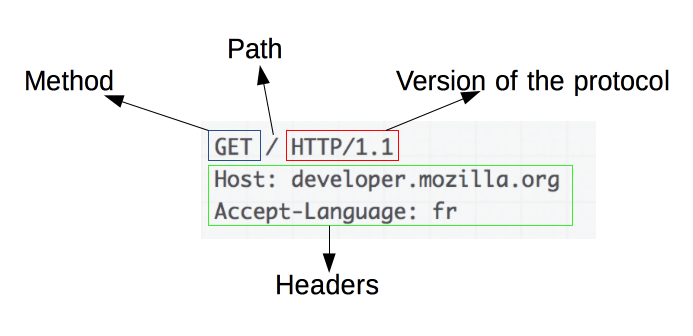
\includegraphics[width=0.7\textwidth]{./images/chapter2/http_request.png}
	\caption[Βασική Δομή ενός αιτήματος http]{Βασική Δομή ενός αιτήματος http}
	\label{fig:http_request}
\end{figure}

\subsection{Μέθοδοι}
\label{subsec:http_methods}

Πιο συγκεκριμένα οι βασικές μέθοδοι που παρέχει το http και οι συνήθεις λειτουργίες τους είναι οι εξής:

\begin{itemize}
	\item \textbf{GET}: παίρνει πληροφορία από τον server
	\item \textbf{POST}: υποβάλλει πληροφορία, προκαλώντας αλλαγές στον τρόπο λειτουργίας του server. Σχετίζεται συχνά με τη δημιουργία πληροφορίας που προηγουμένως δεν υπήρχε 
	\item \textbf{PUT}: όπως και πριν στέλνει πληροφορία στον παραλήπτη υπολογιστή, αλλά αυτή τη φορά επηρεάζει πόρους που ήδη υπήρχαν στο σύστημα. Σχετίζεται συχνά με την τροποποίηση ήδη υπάρχουσας πληροφορίας
	\item \textbf{DELETE}: διαγράφει από το σύστημα του server το συγκεκριμένο πόρο.
\end{itemize}

Αξίζει να σημειωθεί ότι πέρα από τις τέσσερις αυτές βασικές μεθόδους υπάρχουν και άλλες όπως είναι 
η \textbf{PATCH} που αποτελεί ειδική περίπτωση της PUT, η \textbf{HEAD} που αποτελεί ειδική περίπτωση της GET,
καθώς και άλλες που σχετίζονται με τη σύνδεση μεταξύ server και client. Αυτές είναι οι \textbf{CONNECT}, \textbf{OPTIONS} και \textbf{TRACE}.
Καθώς όμως, οι υπόλοιπες αυτές οι μέθοδοι, δεν χρησιμοποιούνται τόσο συχνά στην πράξη, δεν θα αναλυθούν περαιτέρω.

\subsection{Εκδόσεις HTTP}
\label{subsec:http_versions}

Η πρώτη έκδοση του HTTP, παρόλλο που δεν είχε κάποια συγκεκριμένo τίτλο, εκ των υστέρων ονομάστηκε 
HTTP/0.9. Αποτελεί την πιο απλή έκδοση του πρωτοκόλλου. Δεν υποστηρίζονταν headers και κωδικοί κατάστασης (status codes).
Εξυπηρετούσε μόνο GET αιτήματα και η μοναδική απάντηση που μπορούσε να επιστρέψει ήταν hypertext αρχεία. Kάθε φορά που ο server ανταποκρινόταν και έστελνε
απάντηση, η επικοινωνία με τον client έκλεινε κατευθείαν.

Στη συνέχεια και με την ανάπτυξη του διαδικτύου προστέθηκαν και άλλες λειτουργίες. Πέριξ του 1996,
με τη επόμενη έκδοση του πρωτοκόλλου (HTTP/1.0) τα αιτήματα πλέον συνοδεύονταν από headers, μεταπληροφορία σχετικά
με τη κατάσταση του αιτήματος, τον τύπο της πληροφορίας που περιμένουμε να έρθει (stylesheets, media, hypertext) καθώς και 
την έκδοση του HTTP που χρησιμοποιήθηκε στη συγκεκριμένη επικοινωνία. Επιπλέον πέρα από τη GET μέθοδο υπάρχει η
δυνατότητα για POST και PUT, δημιουργία και τροποποίηση πληροφορίας δηλαδή.

Στη συνέχεια το HTTP/1.1 προσπαθεί να βελτιώσει τις ήδη υπαρχουσες δυνατότητες κάνοντας την επικοινωνία
μεταξύ server και client πιο αποδοτική. Αντί να κλείνει η επικοινωνία μετά από κάθε μήνυμα, η σύνδεση παραμένει
ανοιχτή γλιτώνοντας έτσι μία σταθερή καθυστέρηση που υπήρχε σε κάθε αίτημα

Φτάνοντας στο σήμερα, μιλάμε για το HTTP/2.0 \cite{http2}. Αξιοποιώντας το πρωτόκολλο Speedy (SPDY) που αναπτύχθηκε κάποια χρόνια πριν
την κυκλοφορία του, και κτίζοντας πάνω σε αυτό, κατάφερε να μειώσει τους χρόνους επικοινωνίας server-client.
Μερικοί από τους τρόπους που επιτυγχάνεται αυτό είναι η μετατροπή του http από text πρωτόκολλο, σε δυαδικό (binary protocoll), επιτρέποντας έτσι χρήση καλύτερων
και αποδοτικότερων τεχνικών επικοινωνίας. Επιπλέον συμπιέζει τους headers (header compression) καθώς αποτελούν πληροφορία που
επαναλαμβάνεται όταν τα αιτήματα στον server είναι συνεχή. Ο server ακόμα, αποκτά έναν μηχανισμό (server-push) που του
επιτρέπει να προωθεί πληροφορία στον client (στην cache του client συγκεκριμένα), που δεν έχει ζητήσει ακόμα, αλλά βάση αυτού
που αιτήται, μάλλον θα ζητήσει εντός της ιδίας συνεδρίας.

Τέλος, πρέπει να αναφερθούμε στην τελευταία, αν και όχι ακόμα ευρέως διαδεδομένη, έκδοση HTTP/3.0. H βασική διαφορά με τους
πρωκατόχους του είναι ότι αλλάζει το πρωτόκολλο επικοινωνίας που χρησιμοποιεί όλα αυτά τα χρόνια, από TCP (Transfer Communication Protocoll) σε
έναν συνδυασμό UDP (User Datagram Protocoll) και QUIC (Quick UDP Internet Connections), μίας νέας τεχνολογίας που λύνει το πρόβλημα και βελτιστοποιεί τόσο το πρόβλημα 
της ασφάλειας των επικοινωνιών (TLS handshakes), όσο και της απώλειας πληροφορίας που μπορεί να υπήρχε λόγω UDP, πρωτοκόλλου που είναι γνωστό
για την ταχύτερη απόδοσή του σε σχέση με το TCP, αλλά και το γεγονός ότι είναι πιο επιρρεπές σε σφάλματα. Η νέα αυτή έκδοση από τα αποτελέσματα 
του \cite{http3} φαίνεται να έχει ήδη καλύτερους χρόνους σε σχέση με τις παλαιότερες εκδόσεις και ήδη το 28\% του διαδικτύου αξιοποιεί τις δυνατότητές του. 


\subsection{Κωδικοί Κατάστασης}
\label{subsec:http_status_codes}

Οι κωδικοί κατάστασεις (status codes) αποτελούν μέρος της απάντησης του server. Επιτρέπουν στον χρήστη να καταλάβει με μία ματιά αν το αίτημα που έχει κάνει έχει επιστρέψει σωστά, ή έχει γίνει κάποιο λάθος στη μεριά του server.
Υπάρχουν πέντε μεγαλύτερες κατηγορίες που στεγάζουν όλες τις υποπεριπτώσεις αυτών. Πιο συγκεκριμένα:

\begin{itemize}
	\item \textbf{Εύρος 100-199}: Υποδηλώνουν ενημερωτική απάντηση σχετικά με τη λειτουργία του server
	\item \textbf{Εύρος 200-299}: Επιτυχή αιτήματα. 
	\item \textbf{Εύρος 300-399}: Υποδηλώνουν την ανακατεύθυνση του μηνύματος του client. Συνήθως συνοδεύονται από το νέο url στο οποίο πρέπει να αποσταλλεί το αίτημα
	\item \textbf{Εύρος 400-499}: Ανεπιτυχές αίτημα, που οφείλεται στον client. Ένα σύνηθες παράδειγμα είναι η αίτηση πρόσβασης σε προστατευόμενους πόρους χωρίς κάποιου είδους αυθεντικοποίηση, ή χωρίς τα σωστά στοιχεία για αυθεντικοποίηση
	\item \textbf{Εύρος 500-599}: Ανεπιτυχές αίτημα, που οφείλεται στον server. 
\end{itemize}
% \input{./chapters/chapter3_theory/section1_dnn.tex}
% \input{./chapters/chapter3_theory/section2_cnn.tex}
% \input{./chapters/chapter3_theory/section3_sota.tex}
\newevenside

% % chapter 3 = State of the art
% - αναφορά σε commercial και open source projects
% - παράθεση πλεονεκτημάτων της δικής μου υλοποίησης (βασικά εδώ αναφέρουμε τα: 
% (1)infinite scalability και ίσως το γεγονός ότι μπορούμε να (
% (2) κοιτάμε σε μεγάλο βάθος χρόνου για να παρουσιάσουμε "συνολικά στατιστικά", χωρίς αυτό να επιβαρύνει τη βάση μας ή να δυσχαιρένει τη λειτουργία του συστήματος μας). 
% Το γεγονός ότι έχει infinite scalebility μας παρέχει τη δυνατότητα να έχουμε
% (3)όσα 1m intervals θέλουμε και ακόμα τη δυνατότητα να κάνουμε stress test με όσα requests per minute θέλει ο χρήστης.
% Tέλος τα περισσότερα ενώ κάποια από αυτά τασ εργαλεία σου δίνουν τη δυνατότητα να κάνεις customise τα μηνυματα που στέλνεις,
% τα περισσότερα δε σε αφήνουν να τροποποιήσεις τα apis σου.

% commercial products - Better Uptime, Pulsetic, Datadog, Freshping, Hyperping, UptimeRobot
% open souce - Upptime, Uptime Kuma, Cabot, Zabbix, Sensu

\chapter{Βιβλιογραφική Αναζήτηση Τεχνολογιών Αιχμής}
\label{chapter:state_of_the_art}

Πριν αναλυθεί η υλοποίηση του συστήματος που δημιουργήσαμε για την Ενεργή Παρακολούθηση
Eφαρμογών ως Υπηρεσίες (SaaS) και ιστοσελιδών που εδρεύουν στο διαδίκτυο, θα πασουσιάσουμε τεχνολογίες
που έχουν χτιστεί ήδη για τον σκοπό αυτό και θα δείξουμε τους τομείς στους οποίους
διαφέρει το δικό μας σύστημα.

Εφαρμογές τέτοιου τύπου έχουν αναπτυχθεί κυρίως από εταιρίες, αλλά υπάρχουν πολλά open source
projects μικρότερου βεληνεκούς που επιτυγχάνουν τον ίδιο στόχο. Στη συνέχεια θα αναφερθούμε κυρίως στα
πιο γνωστά και διαδεδομένα εργαλεία, παρουσιάζοντας τα δυνατά τους σημεία και περιγράφοντας τις λειτουργίες
που παρέχουν.

\begin{itemize}
	\item \textbf{Better Uptime}: Προσφέρει εύκολη ενσωμάτωση των ιστοσελιδών που θέλει κανείς να παρακολουθήσει.
	      Λειτουργεί κάνοντας ping κάθε τριάντα δευτερόλεπτα στο url που ορίζει ο χρήστης και παρουσιάζει
	      τα παραγόμενα δεδομένα σε ευπαρουσίαστα διαγράμματα (\autoref{fig:better_uptime}). Ένα από τα μεγάλα πλεονεκτήματα που έχει αφορά
	      τη δυνατότητα για πολλαπλά ping από διαφορετικές περιοχές του κόσμου (Ευρώπη, Ασία, Βόρεια Αμερική, Αυστραλία),
	      ώστε οι χρήστες να διαθέτουν μία πιο πλήρη εποπτεία του υπό μελέτη συστήματος/ιστοσελίδας. Αξίζει να σημειωθεί
	      ότι παρέχει και μηχανισμούς ενημέρωσης για να ειδοποιεί το χρήστη σε περίπτωση μη απόκρισης τους συστήματος, μέσα
	      από mail, εφαρμογές chatting και τηλεφωνικών κλήσεων.
	      \begin{figure}[!ht]
		      \centering
		      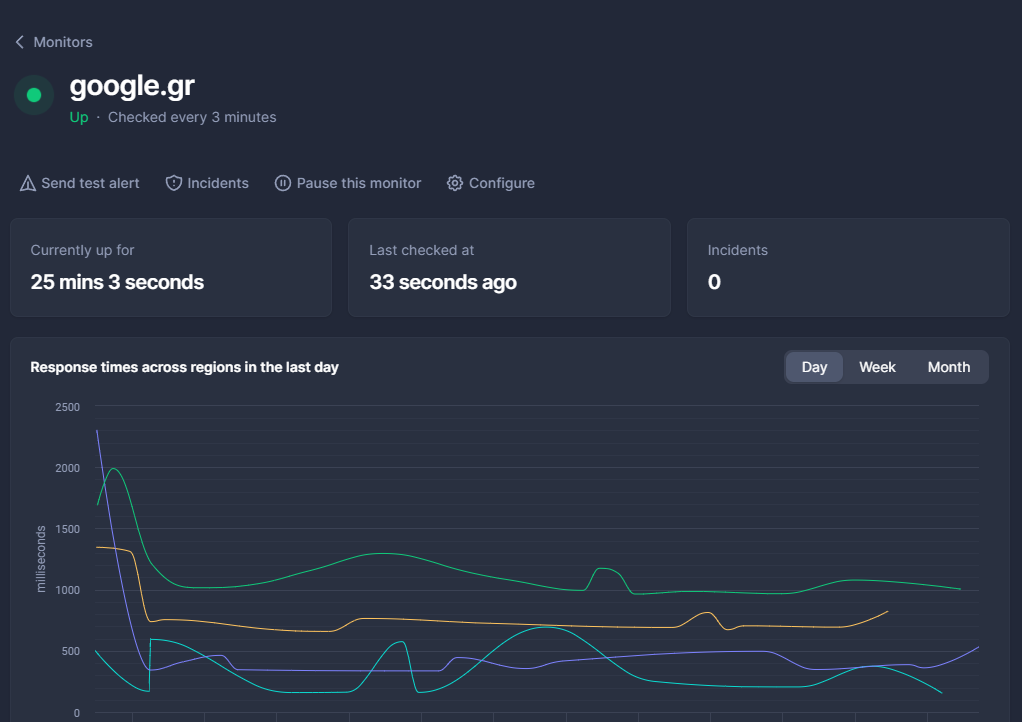
\includegraphics[width=0.7\textwidth]{./images/chapter3/better-uptime-cropped.png}
		      \caption[Παράδειγμα χρήσης του εργαλείου Better Uptime]{Παράδειγμα χρήσης του εργαλείου Better Uptime}
		      \label{fig:better_uptime}
	      \end{figure}
	\item \textbf{Uptime Robot}: Επιτρέπει, πέρα από την επιλογή του url, και την επιλογή παραπάνων παραμέτρων που επηρεάζουν
	      την απάντηση που θα επιστρέψει το υπό μελέτη σύστημα. Οι παράμετροι αυτοί σχετίζονται με τους headers του μηνύματος που
	      αποστέλλεται, και πιο συγκεκριμένα, με αυτούς που αφορούν την αυθεντικοποίηση του χρήστη (στην προκειμένη περίπτωση
	      του συστήματος παρακολούθησης). Πέρα από αυτά μπορεί να καθορίσει την επιθυμητή http κατάσταση της απόκρισης
	      της ιστόσελίδας και το χρόνο που θα παρεμβάλλεται μεταξύ διαδοχικών αιτημάτων (pings). Τέλος, διαθέτει κάποια βασικά διαγράμματα
	      που σχετίζονται με το αν η απόκριση του συστήματος είναι ορθή ή όχι (\autoref{fig:uptime_robot})
	      \begin{figure}[!ht]
		      \centering
		      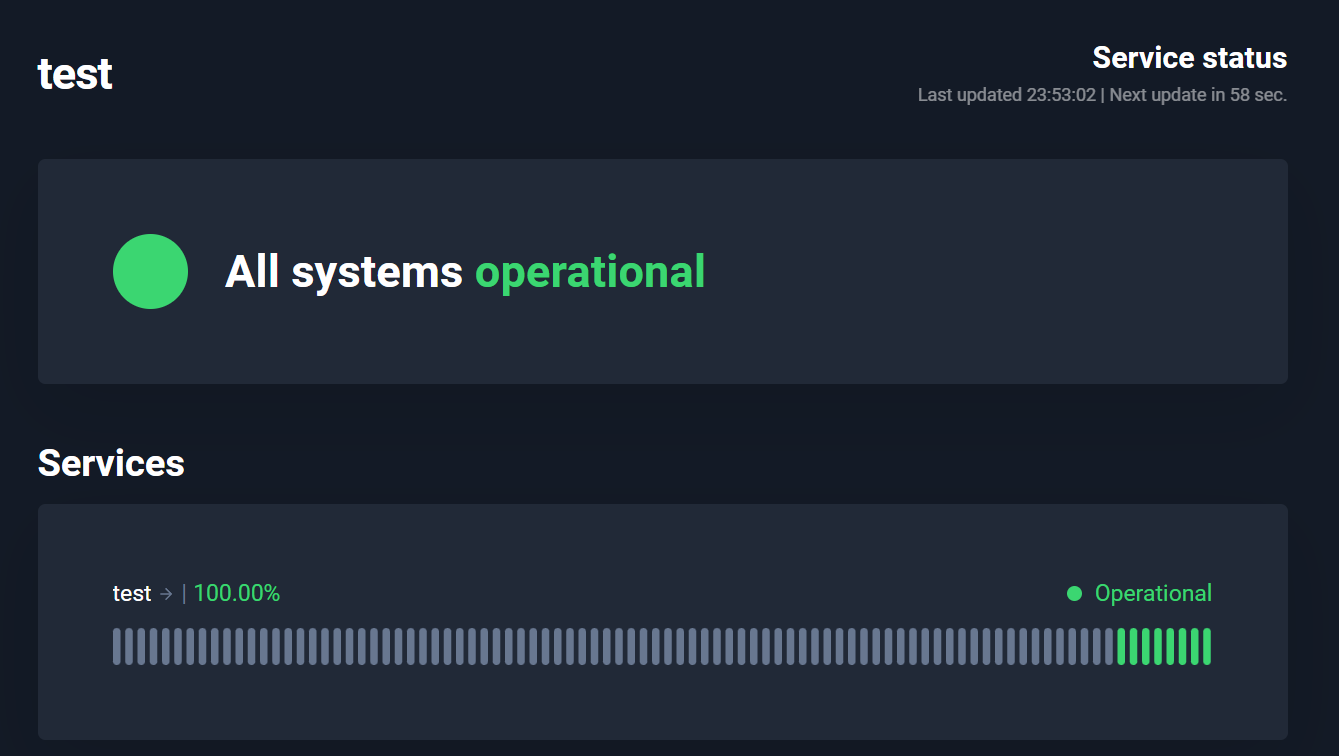
\includegraphics[width=0.7\textwidth]{./images/chapter3/uptime_robot.png}
		      \caption[Παράδειγμα χρήσης του εργαλείου Uptime Robot]{Παράδειγμα χρήσης του εργαλείου Uptime Robot}
		      \label{fig:uptime_robot}
	      \end{figure}
	\item \textbf{Site24x7}: Διαθέτει μετρικές, που αφορούν τη μέγιστη/ελάχιστη τιμή του χρόνου απόκρισης του συστήματος, καθώς και τη μέση τιμή του,
	      ενώ παράλληλα δίνει μία εικόνα του throughput του συστήματος. Δεν λείπει φυσικά και ένα διάγραμμα απόκρισης χρόνου (\autoref{fig:site24x7})
	      που καθιστα τα δεδομένα που συλλέγονται πιο εύκολα στην κατανόηση και οπτικοποίηση.
	      \begin{figure}[!ht]
		      \centering
		      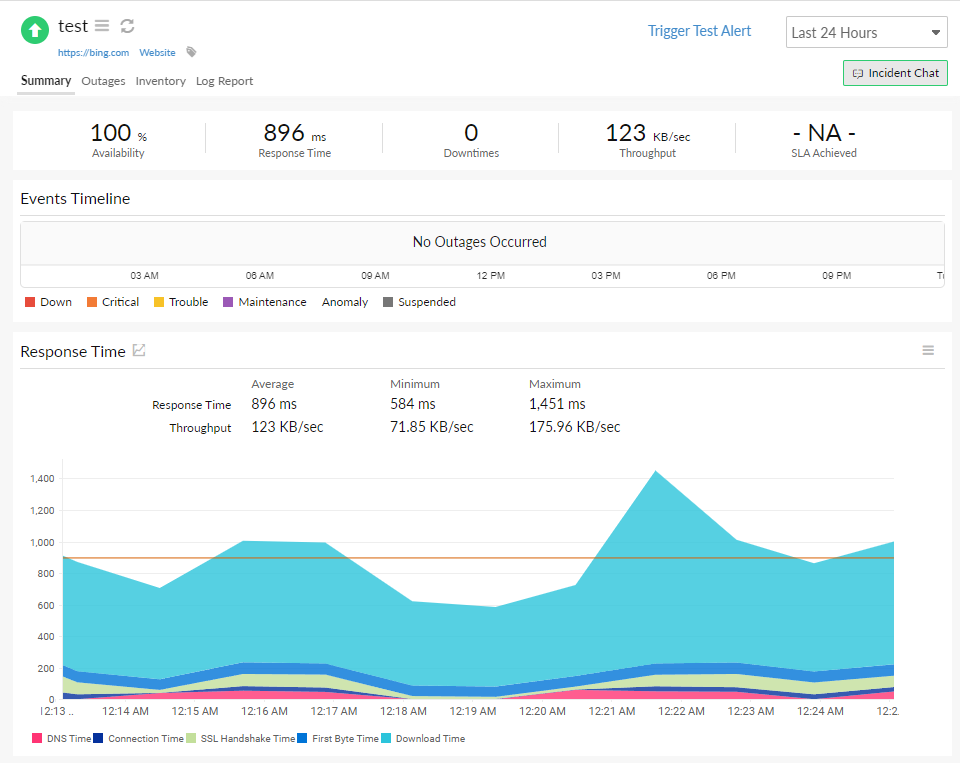
\includegraphics[width=0.7\textwidth]{./images/chapter3/site24x7.png}
		      \caption[Παράδειγμα χρήσης του εργαλείου Site24x7]{Παράδειγμα χρήσης του εργαλείου Site24x7}
		      \label{fig:site24x7}
	      \end{figure}
	\item \textbf{Uptimia}: Πέρα από τα κλασικού τύπου http αιτήματα, μπορεί να κάνει ελέγχους παρακολούθησης (uptime monitoring)
	      σε DNS, UDP, TCP και email με απόσταση έως και τριάντα δευτερολέπτων (μεταξύ αιτημάτων). Αξίζει, να σημειωθεί, ότι η συγκεκριμένη
	      εφαρμογή έχει δυνατότες και παθητικής παρακολούθησης (RUM). Αρχικά επιλέγεται το site το οποίο ο χρήστης θέλει να παρακολουθήσει, καθώς και τα δεδομένα για το οποία επιθυμεί να ενημερώνεται ή να παρακολουθεί.
		  Αυτά σχετίζονται, κυρίως με σφάλματα ή καταστάσεις στις οποίες βρίσκεται το σύστημα και μπορεί να δηλώνουν κάποιο πρόβλημα.
		  Καταστάσεις όπως είναι η μειωμένη απόδοση του υπό μελέτη συστήματος ή η απότομη πτώση του πλήθους των χρηστών μίας σελίδας.
	      Για να επιτύχει τέτοιας μορφής ελέγχους, παράγει (ανάλογα με τον τύπο των ελέγχων που επιλέγουμε)
	      ένα script γραμμένο σε JavaScript που τοποθείται στην αρχή της ιστοσελίδας την οποία θέλουμε να παρακολουθήσουμε.
	      Με αυτό τον τρόπο δίνεται η δυνατότητα συλλογής δεδομένων πραγματικών χρηστών.
	      \begin{figure}[!ht]
		      \centering
		      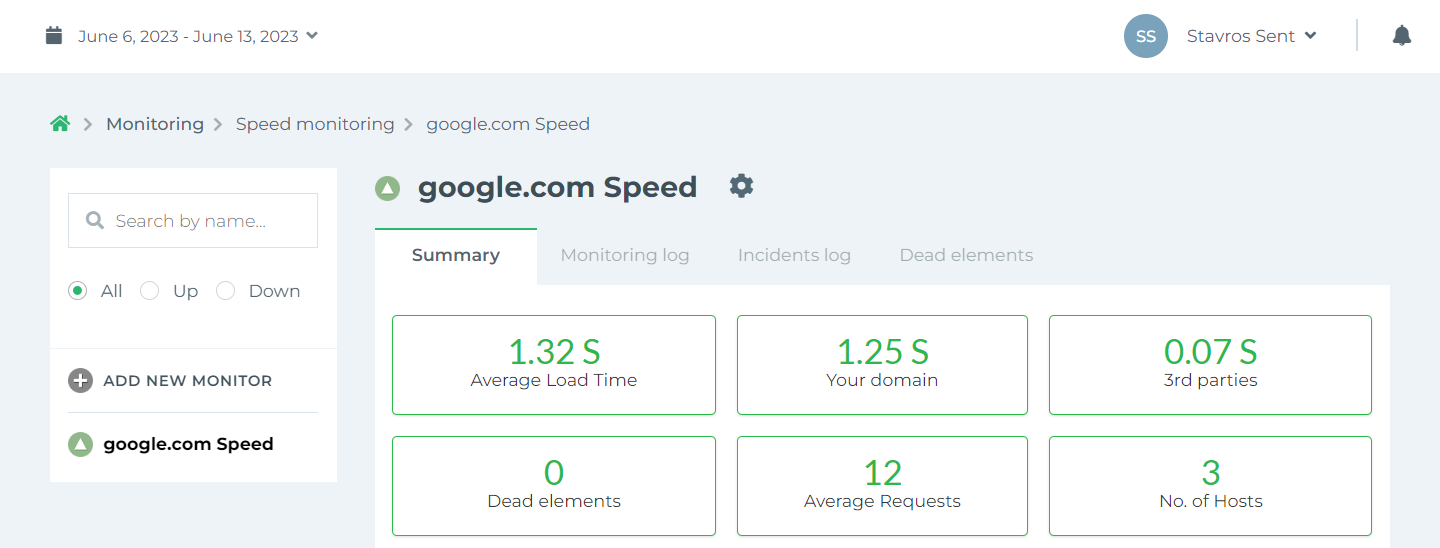
\includegraphics[width=0.7\textwidth]{./images/chapter3/uptimia.png}
		      \caption[Παράδειγμα χρήσης του εργαλείου Uptimia]{Παράδειγμα χρήσης του εργαλείου Uptimia}
		      \label{fig:uptimia}
	      \end{figure}
\end{itemize}

\break

Παραπάνω αναφέρθηκαν μερικά μόνο κάποια από τα εργαλεία που υπάρχουν σήμερα για την Ενεργη Παρακολούθηση του Χρόνου
και Απόκρισης Ιστοτόπων και Διαδικτυακών Εφαρμογών. Σε αυτά θα πρέπει να προστεθούν πληθώρα εφαρμογών όπως τα:
\textbf{StatusCake}, \textbf{SemaText}, \textbf{Uptrends}, \textbf{Dotcom-monitor}, \textbf{Updown}, \textbf{Datadog Synthetics}.
Οι δυνατότες που προσφέρουν ως επί το πλείστον μπορούν περιγραφούν πλήρως από όσα αναπτύξαμε προηγουμένως, για αυτό το λόγω δεν θα αναφερθούμε περαιτέρω.

Πρέπει σε αυτό το σημείο όμως, να τονίσουμε ότι όσα προαναφέρθηκαν αποτελούν προϊόντα εταιριών.
Αυτό όμως δεν σταματάει την ανάπτυξη open source projects που υλοποιήθηκαν από χρήστες είτε ως προσωπικά projects, είτε
ως projects μίας μεγαλύτερης ομάδας από developers. Έτσι και στο πλαίσιο της Ενεργής Παρακολούθησης μερικά από τα πιο
γνωστά και δημοφιλή μεταξύ developers αποθετήρια αποτελούν τα:

\begin{itemize}
	\item \href{https://github.com/upptime/upptime}{Upptime\footnote{αποθετήριο κώδικα Upttime: \textit{https://github.com/upptime/upptime}}}: Αποτελεί μία ενδιαφέρουσα προσέγγιση στο πρόβλημα
	      της διαχείρησης των schedulers που θα πρέπει να έχει το σύστημα για να κάνει αιτήματα ανά ένα συγκεκριμένο
	      και σταθερό χρονικό διάστημα. Προκειμένου να επιτύχει κάτι τέτοιο αξιοποιεί τις δυνατότητες του GitHub (cloud-based υπηρεσία αποθήκευσης git αποθετηρίων)
	      και των actions που αυτό σου επιτρέπει να εκτελείς κάθε πέντε λεπτά. Έτσι λοιπόν ανά πέντε λεπτά (ελάχιστος χρόνος ελέγχου απόκρισης)
	      τρέχει αυτοματοποιημένα και μέσω του GitHub (ανεξάρτητα από το σύστημα αυτό) μία διαδικασία που κάνει αιτήματα στην σελίδα που ο χρήστης ορίζει.
	      Φυσικά τα αποτελέσματα αυτά αποθηκεύονται και ανά έξι ώρες παράγονται διαγράμματα που μπορείς να τα δεις μέσα από μία σελίδα που παράγεται αυτόματα.
	      \begin{figure}[!ht]
		      \centering
		      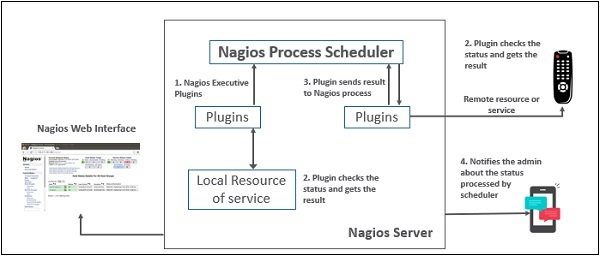
\includegraphics[width=0.8\textwidth]{./images/chapter3/nagios.jpg}
		      \caption[Αρχιτεκτόνική Συστήματος Nagios]{Αρχιτεκτόνική Συστήματος Nagios}
		      \label{fig:nagios}
	      \end{figure}
	\item \href{https://github.com/NagiosEnterprises/nagioscore}{Nagios\footnote{αποθετήριο κώδικα Nagios: \textit{https://github.com/NagiosEnterprises/nagioscore}}}: Είναι ένα πρόγραμμα γραμμένο στη γλώσσα προγραμματισμού
	      C. Πέρα από το backend διαθέτει και Γραφικό Περιβάλλον Χρήστη (Graphical User Interface - GUI).
	      Αποτελείται από ένα σύστημα ενός server (nagios server), o oποίος λειτουργεί σαν ένας scheduler που στέλνει σήματα
	      για να ξεκινήσει την εκτέλεση plugins στα απομακρυσμένα συστήματα που θέλουμε να παρακολουθήσουμε. Μόλις τα plugins δεχτούν
	      απάντηση επιστρέφουν στον server o οποίος προωθεί την πληροφορία στο GUI για να τη δούνε και οι χρήστες. Δεν χρησιμοποιείται κάποια βάση
	      δεδομένων, καθώς η πληροφορία που μαζεύεται αποθηκεύεται μόνο σε logs στο σύστημα που τρέχει την υπηρεσία αυτή. Την αρχιτεκτονική σου συστήματος μπορούμε
		  δούμε στo \autoref{fig:nagios}
	\item \href{https://github.com/louislam/uptime-kuma}{Kuma Uptime\footnote{αποθετήριο κώδικα Kuma Uptime: \textit{https://github.com/louislam/uptime-kuma}}}: Αποτελεί μία εύκολή, στη χρήση και στήσιμο,
	      self-hosted εφαρμογή γραμμένη σε JavaScript για Ενεργή Παρακολούθηση. Για την αποστολή των αιτημάτων σε απομακρυσμένες (στο διαδίκτυο) σελίδες
	      χρησιμοποιεί \textbf{child\_proccesses}, ένα api δήλαδή που περιλαμβάνει η Node.js για τη δημιουργία διεργασιών (processes) εντός άλλων διεργασιών.
	      Η εφαρμογή περιλαμβάνει backend και frontend, στο οποίο εμφανίζονται τα αποτελέσματα του monitoring. Αξίζει να σημειωθεί
	      ότι τα δεδομένα αποθηκεύονται σε βάση SQLite, ένα προσωρινό σύνολο δεδομένων που υφίσταται μόνο στο πλαίσιο εκτέλεσης μίας εφαρμογής.
	      Αποτελεί μία server-less βάση δεδομένων και είναι άρρηκτα συνδεδεμένη με την εφαρμογή στην οποία υπάρχει.
	      \begin{figure}[!ht]
		      \centering
		      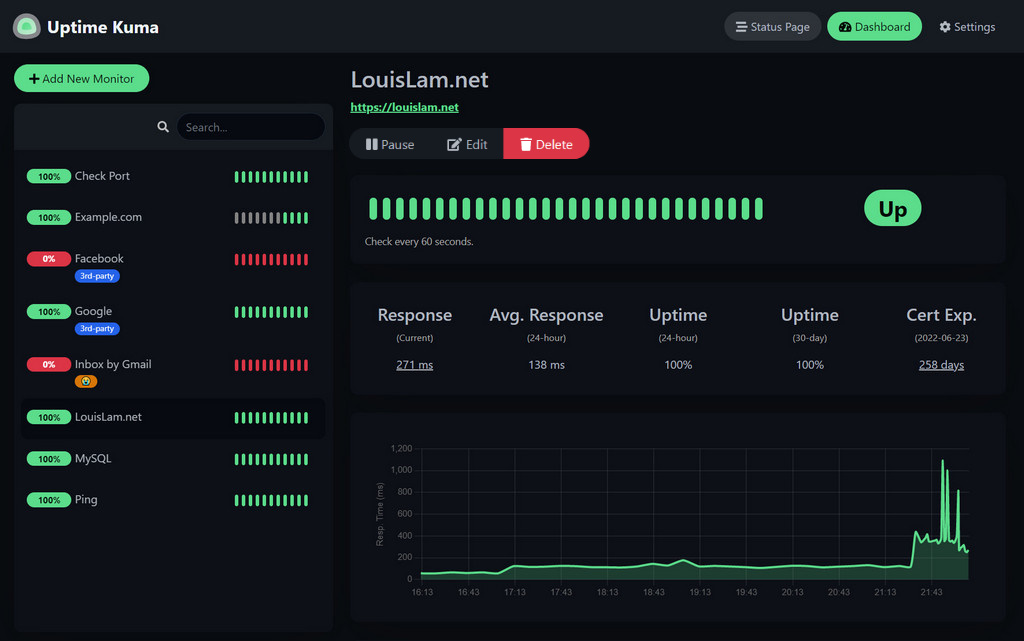
\includegraphics[width=0.7\textwidth]{./images/chapter3/kuma-uptime.jpg}
		      \caption[Παράδειγμα χρήσης του εργαλείου Kuma Uptime]{Παράδειγμα χρήσης του εργαλείου Kuma Uptime}
		      \label{fig:kuma_uptime}
	      \end{figure}
\end{itemize}

Κάθε σύστημα που αναφέρθηκε έχει πλεονεκτήματα αλλά και μειονεκτήματα σε σχέση με άλλα.
Αυτό που θα θέλαμε να διαθέτει ιδανικά ένα σύστημα Παρακολούθησης, βάσει όλων αυτών που είδαμε μέχρι τώρα,
είναι τα εξής:

\begin{enumerate}
	\item Σταθερό και Αξιόπιστο σύστημα διαχείρησης προγραμματισμού (scheduling system) που θα
		καθορίζει το πότε πρέπει να ξεκινάνε τα αιτήματα προς τα εξωτερικά υπό παρακολούθηση συστήματα.
	\item Κάποια μορφή βάσης δεδομένων στην οποία θα αποθηκεύουμε τα δεδομένα που συλλέγουμε.
	\item Χρήση ιστορικών δεδομένων για τον υπολογισμό μετρικών στατιστικής φύσης σε βάθος χρόνου.
	\item Προβολή των δεδομένων σε ευπαρουσίαστα και εύπεπτα διαγράμματα που θα βοηθούν το χρήστη να αντιλαμβάνεται
		γρήγορα την κατάσταση των συστημάτων του
	\item Διάθεση τρόπων ειδοποίησης του χρήστη σε περίπτωση που κάποιο από τα συστήματα δεν ανταποκρίνεται
	\item Δυνατότητα για οριζόντια κλιμάκωση (\textbf{horizontal scaling})
	\item Ελαχιστοποίηση downtime του συστήματος 
	\item Πλήρης παραμετροποίηση του μηνύματος που αποστέλλεται (κατάλληλη ρύθμιση headers, body και query)
	\item Ρύθμιση του χρόνου μεταξύ διαδοχικών μηνυμάτων
\end{enumerate}

Πολλές απο τις εφαρμογές που είδαμε καλύπτουν σε κάποιο βαθμό μερικά από τα παραπάνω, αλλά καμία
δεν τα καλύπτει όλα ταυτόχρονα. Τα εργαλεία που αναπτύχθηκαν στο πλαίσιο εταιριών έχουν δυνατότητες κλιμάκωσης
αλλά στα περισσότερα (αν όχι σε όλα) μπορείς να δεις πληροφορία μέχρι ένα συγκεκριμένο χρονικό διάστημα πίσω στο χρόνο,
κρύβοντας δεδομένα που είτε δεν αποθηκεύουν πλέον είτε δεν μπορούν να αντλήσουν αρκετά γρήγορα.
Απο την άλλη οι περισσότερες open source εφαρμογές που αναφέραμε δεν μπορούν να κάνουν τόσο εύκολα scaling
καθώς είναι φτιαγμένες να δουλεύουν για περιορισμένο πλήθος χρηστών. 

\begin{table}[H]
	\begin{center}
		\caption{Σύγκριση Εργαλείων Ενεργής Παρακολούθησης}
		\label{tab:active_monitoring_characteristics}
		\begin{tabular}{| p{40mm} | c | c | c | c | c | c |}
			\hline & \thead{Τρέχουσα \\ Διπλωματική} & \thead{Better \\ Uptime} & \thead{Uptime \\ Robot} & \thead{Site24x7} & \thead{Uptimia} & \thead{Kuma} \tabularnewline
			\hline \thead{Σταθερότητα} & \checkmark & \checkmark & \checkmark & \checkmark & \checkmark & \checkmark \tabularnewline
			\hline \thead{Βάση Δεδομένων} & \checkmark  & \checkmark  & \checkmark & \checkmark & \checkmark & \tabularnewline
			\hline \thead{Ιστορικά Δεδομένα} & \checkmark & & & & & \tabularnewline
			\hline \thead{Διαγράμματα} & \checkmark & \checkmark & & \checkmark & \checkmark & \tabularnewline
			\hline \thead{Ειδοποιήσεις} & \checkmark & \checkmark & \checkmark & \checkmark & \checkmark & \checkmark \tabularnewline
			\hline \thead{Ελαχιστοποίηση \\ Downtime} & \checkmark & \checkmark & \checkmark & \checkmark & \checkmark & \checkmark \tabularnewline
			\hline \thead{Παραμετροποίηση \\ μηνυμάτων} & \checkmark & \checkmark & \checkmark & \checkmark & \checkmark & \tabularnewline
			\hline \thead{Ρύθμιση Χρόνου \\ μεταξύ μηνυμάτων} & \checkmark & \checkmark & \checkmark & \checkmark & \checkmark & \checkmark \tabularnewline
			\hline \thead{Οριζόντια \\ Κλιμάκωση} & \checkmark & \checkmark & \checkmark & \checkmark & \checkmark & \tabularnewline
			\hline
		\end{tabular}
	\end{center}
\end{table}

Στη διπλωματική αυτή εργασία λοιπόν καλούμαστε να δημιουργήσουμε ένα τέτοιο υπολογιστικό σύστημα
που θα καλύπτει τα προαναφερθέντα.

\newevenside

% % chapter 4 = Υλοποίηση του συστήματος
% 1η Υλοποίηση - Χρήση απλών schedulers και ενός express server που κρατούσαν όλα τα requests μόνο όσο "ζούσε" ο server.
% 2η Υλοποίηση - Προσθήκη στο προηγούμενο ενός κοινού σημείου (socket.io). Σε αυτή την υλοποίηση θα υπήρχαν 1server με τον οποιό θα "επικοινωνούσε" ο χρήστης και πολλοί server "clients" που θα μιλούσαν με τον αρχικό. Η χρήση websockets/socket.io θα ήταν εξαιρετική, καθώς θα μπορούσε σε κάποιες περιτπώσεις να οφελεί η αμφίφρομη εποικοινωνία server και worker, αλλά το γεγονός ότι οι περισσότερες επικοινωνίες θασ είναι μονόδρομες μάλλον μας ωθεί να χρησιμοποιήσουμε έναν κλασικό http server. Επίσης το scaling ενός websocket server είναι αρκετά πιο περίπλοκο και δύσκολο στη συντήρηση.
% 3η Υλοποίηση - Χρήση ενός ή περισοοτέρων (εφόσον χρειαστεί) server και ένας ή περισσότερη workers (scalable). Η κεντρικός server εξυπειρετεί μόνο την επικοινωνία μεταξύ worker και χρήστη και είναι υπεύθυνος για τη δημιουργία, καταστροφή, τροποποίηση ήδη υπάρχοντων jobs. Κάθε worker έχει το δικό του scheduler και εκτελεί τα δικά του jobs/apis καθώς και ένα cleanup jobs μία φορά τη βδομάδα που κάνει Upload τα raw responses, κάποια χρήσιμα στοιχεία σε ξεχωριστά αρχεία καθώς και υπολογίζει/επαναυπολογίζει χρήσιμες στατιστικές τιμές για κάθε μέρα (εδώ αναφορά στο πως περίπου λειτουργεί ο scheduler και εξήγηση της λειτουργίας του άμα "πέσει")

% 1ή υλοποίηση - η πιο απλή και μη λειτουργική. Ένας node server. Κάθε φορά που έρχεται qpi request σηκώνει καινούργιο setInterval με συγκεκριμένο interval κάθε φορά. Ιδανικό γιατί δεν θα έχεις ποτέ πρόβλημα με τον χρόνο
% 	μεταξύ διαδοχικών request επειδή είναι ακριβές. Κακή απόδοση όταν ο αριθμός των request αυξηθεί πάρα πολύ. Ξεχωριστά timer αυξάνουν την πολυπλοκότητα. Επίσης θα υπάρχει πρόβλημα όταν "πέφτει" ο server εξαιτίας κάποιου πιθανού
%	προβλήματος. Ακόμα και να κρατάμε τα jobs σε κάποια βάση δεν θα ξέρουμε πότε πρέπει να ξανατρέξουν. Αν πχ έχεις κάποιο
%	api να τρέχει κάθε 30s και μόλις εκτελεστεί "πεσει" ο server. Τότε θα πρέπει είτε να μην ξεκινήσεις το job και να χάσεις πιθανώς ένα request
% 	είτε να τρέξεις το job ότν και να γίνει και να έχεις διπλοεγγραφές.

% 2ή υλοποίηση - ένας node http και socketio/server και ένας ή παραπάνω socketio/client server. O main server θα είναι υπεύθυνος για το routing
%	των apis και οι υπόλοιποιν θα λαμβάνουν μηνυματα και θα τα εκτελούν ξεκινώντας πάλι setIntevral με συγκεκριμένα interval το καθένα
%	έτσι λύνται το πρόβλημα του πιθανού overload του main server. Ο λόγος χρήσης websockets είναι για να έχεις πιο γρήγορη και άμεση επικοινωνία
%	μεταξύ των server (worker και main) - επικοινωνία που εξυπηρετεί στην επισκόπηση του συστήματος (πόσα μηνύματα έχει κάθε worker) και μαζική μεταφορά μηνυμάτων
%	σε περίπτωση που πέσει κάποιος server. Επίσης websockets εξαιρετικά πιο γρήγορη σε σχέση με http.
%	επίσης επειδή το connection μεταξύ server και worker γίβεται μία φορά γλιτώνεις τα overhead από όλα τα πιθανά http requests που θα έκανες

% 3η υλοποίηση - ένας http server (ή παραπάνω αν χρειαστεί για καλύτερη εξυπηρέτηση) που απλώς servιρουν δεδομένα.
%	worker και server δεν επικοινωνούν μεταξύ τους, αλλά έχοιυν ένα κοινό΄σημείο αναφοράς (db).
% 	κάθε worker έχει ένα όνομα προκειμένου να ξέρει από που θα αντλήσει ποληροφορία
%	μετά ξεκίνα να μιλάς για το πως προκύπτουν τα στατιστικά. Μίλα για cleanup job και το πως ακριβώς λειτουργεί
% 	ανέφερε avro και το πως η standarized μορφή της πληροφορίας που αποθηκεύεται το καθιστά
%	μία πολύ καλή επιλογή για την αποθήκευση της πληροφορίας

\chapter{Υλοποιήσεις}
\label{chapter:implementations}

Στο κεφάλαιο αυτό θα αναφερθούμε στο σύστημα που υλοποιήσαμε προκειμένου να πετύχουμε έναν συνδυασμό Ενεργής-Παθητικής Παρακολούθησης με δυνατότητες αυτόματης διευθέτησης πόρων, με σκοπό τη βελτιστοποίηση των υπό μελέτη συστημάτων. Οι βασικές λειτουργίες του συστήματός μας παρατίθενται παρακάτω:\newline

\textbf{Functional Requirements:}
\begin{itemize}
    \item Το σύστημα θα πρέπει να μπορεί να δέχεται URLs καθώς και άλλες πληροφορίες που κρίνονται απαραίτητες για να μπορεί να τα παρακολουθεί, ανά χρονικά διαστήματα που ορίζει ο χρήστης.
    \item Ο χρήστης θα πρέπει να μπορεί να εισάγει κάποια βασικά στοιχεία για τον έλεγχο που θέλει να προσθέσει (url, χρόνο μεταξύ διαδοχικών ελέγχων) καθώς και περαιτέρω στοιχεία που αφορούν το ίδιο το αίτημα που θα πραγματοποιήσει (προσθήκη authorization headers, εκτιμώμενη απάντηση από το σύστημα για validation) 
    \item Το σύστημα θα πρέπει να διαθέτει λειτουργίες scheduler. Να εκτελεί δηλαδή συγκεκριμένες ρουτίνες ανά συγκεκριμένες χρονικές περιόδους.
    \item Το σύστημα θα πρέπει να μπορεί να συλλέγει μεγάλο όγκο δεδομένων και να κρατάει στατιστικά στοιχεία πάνω σε αυτά.
    \item Το σύστημα θα πρέπει να διαθέτει έναν "έξυπνο" μηχανισμό αναγνώρισης ανωμαλιών στους χρόνους αποκρίσεων που συλλέγει κατά τη διάρκεια λειτουργίας του.
    \item Το σύστημα θα πρέπει να μπορεί να συλλέγει δεδομένα κατανάλωσης πόρων από το ίδιο το μηχάνημα που μελετά απομακρυσμένα, εφόσον αυτό έχει μορφή docker container.
    \item Το σύστημα θα πρέπει να μπορεί να τροποποιεί τους διαθέσιμους πόρους του μηχανήματος που ελέγχεται, εφόσον αυτό έχει μορφή docker container.
\end{itemize}

\textbf{Non-Functional Requirements:}
\begin{itemize}
    \item Το scheduling σύστημα θα πρέπει να εκτελεί της ρουτίνες του εντός ορισμένου χρονικού πλαισίου και να μην αποκλίνει από αυτό
    \item Ο αλγόριθμος αναγνώρισης ανωμαλιών θα πρέπει να μην είναι υπολογιστικά "βαρύς", ώστε να εξυπηρετούνται παράλληλα περισσοτεροι από ένας χρήστες
\end{itemize}\mbox{}\\

Γίνεται εμφανές ότι το παραπάνω σύστημα σπάει σε περισσότερα από ένα υποσυστήματα: 

\begin{itemize}
    \item Έναν node express server που στεγάζει το API του συστήματός μας, μοιράζει τις απαραίτητες λειτουργίες στα υπόλοιπα υποσυστήματα και οργανώνει τη ροή της πληροφορίας.
    \item Έναν scheduler, βασική λειτουργία του οποίου είναι να κάνει ping ανά ορισμένα χρονικά διαστήματα URLs (τα οποία είναι αποθηκευμένα σε μία βάση δεδομένων). Πέραν αυτού διαθέτει και άλλες ρουτίνες οι λειτουργίες των οποίων θα αναλυθούν στη συνέχεια.
    \item Αν το υπό μελέτη σύστημα είναι φτιαγμένο με τεχνολογία Docker τότε προστίθεται ένα ακόμα υποσύστημα σε μορφή docker container, που τρέχει στο ίδιο σύστημα με αυτό που μελετάμε και στέλνει logs για την κατανάλωση πόρων των containers που ελέγχουμε. Το υποσύστημα αυτό τροποποιεί δυναμικά τους διαθέσιμους προς τα containers πόρους ανάλογα με τις εντολές που δέχεται απο το σύστημα που θα αναφερθεί στη συνέχεια. Επειδή το υποσύστημα αυτό λειτουργεί σαν μία διάβαση πεζών αυξάνοντας και μειώνοντας τους πόρους προκειμένου να εχουμε λιγότερο συνοστισμό στο εξής θα αναφέρεται ως \textbf{Krosswalk}
    \item Τέλος ένα υποσύστημα που διαβάζει τους χρόνους αποκρίσεων που μαζεύουν οι schedulers κατα τη λειτουργία τους, και κάνει αναγνώριση ανωμαλιών πάνω στα καινούργια δεδομένα που λαμβάνει κάθε φορά. Το υποσύστημα αυτό στέλνει εντολές στο Krosswalk, κάθε φορά που κρίνει ότι υπάρχει κάποια μη φυσιολογική τιμή στη χρονοσειρά που αναλύει. Το σύστημα αυτό στο εξής θα αναφέρεται ως \textbf{Oracle}. 
\end{itemize}

Πλέον και χάριν συντομίας, στο υπόλοιπο κομμάτι της διπλωματικής αυτής εργασίας, θα αναφερόμαστε στο παραπάνω σύστημα, με το όνομα \textbf{Lychte} (/licht/). Η ονομασία αυτή προκύπτει από τα αρχικά του "\textbf{L}ightweight \textbf{Y}et \textbf{C}onfigura\hyp{}ble \textbf{H}ΤTP \textbf{T}raffic \textbf{E}xpert", που περιγράφει την λειτουργία και μερικά μόνο από τα πολλά χαρακτηριστικά του συστήματος μας.

\section{Server}
\label{section:lychte_server}

Αποτελεί τον "εγκέφαλο" του Lychte. Επικοινωνεί άμεσα και έμμεσα με όλα τα υπόλοιπα υποσυστήματα. Οργανώνει τη ροή της πληροφορίας και διαθέτει api μέσω του οποίου μπορούμε να έχουμε πρόσβαση σε όλη την αποθηκευμένη πληροφορία, εφόσον έχουμε τα κατάλληλα κλειδιά authentication και authorization. Πέρα των προαναφερθέντων υποσυστημάτων επικοινωνεί με μία βάση δεδομένων NoSQL και πιο συγκεκριμένα με μια MongoDB.
Η βάση αυτή επιλέχθηκε λόγω της ικανότητάς της να αποθηκεύει μεγάλο όγκο δεδομένων, ο τύπος σχήματος (schema) των οποίων δεν χρειάζεται να είναι αυστηρά προκαθορισμένος. Επιπλέον οι δυνατότητες που παρέχει για sharding καθώς και για εύκολη και γρήγορη κλιμάκωση την καθιστούν ιδανική για το σύστημα μας, που συνεχώς αποθηκεύει νέα δεδομένα στη βάση.

Συνεχίζοντας στο πλαίσιο της βάσης δεδομένων έχουμε ορίσει ορισμένες οντότητες (collections) για την πιο εύκολη αποθήκευση και οργάνωση της πληροφορίας:

\begin{itemize}
    \item \textbf{Api} (\autoref{fig:api_doc}): περιέχει αποθηκευμένες πληροφορίες για τον έλεγχο που θέλουμε να υλοποιήσουμε. Σε αυτές περιλαμβάνονται:
        \begin{itemize}
            \item Μοναδικό ID που περιγράφει μονοσήμαντα το συγκεκριμένο API
            \item Tίτλος
            \item URL
            \item H μέθοδος του url που θέλουμε να ελέγξουμε (GET, POST, PUT, DELETE, PATCH)
            \item O τύπος της αναμενόμενης απάντησης (JSON, STREAM, TEXT)
            \item Ο χρόνος μεταξύ των διαδοχικών ελέγχων
            \item Query παράμετροι που θα στείλουμε μαζί με το url
            \item Body που θα στείλουμε υπό μορφή json στις περιπτώσεις των POST, PUT, DELETE, PATCH αιτημάτων
            \item Headers
            \item Status Code: Το ορίζει ο χρήστης προκειμένου να μπορεί να γίνει έλεγχος αν το αίτημα επιστρέφει αυτό που κανονικά θα έπρεπε
            \item Response body υπό μορφή json: Ομοίως ορίζεται από τον χρήστη για τον λόγο που προαναφέρθηκε 
        \end{itemize}
    \item \textbf{Response} (\autoref{fig:response_docs}): περιέχει αποθηκευμένες πληροφορίες από τα αιτήματα που κάνουμε στα αποθηκευμένα στη βάση apis. Σε αυτά αποθηκεύουμε:
        \begin{itemize}
            \item Το id από το api για το οποίο έχει πραγματοποιηθεί το αίτημα
            \item Ένα πεδίο hasError που περιγράφει το αν το αναμενόμενο (αυτό που έχει ορίσει ο χρήστης) response διαφέρει από το συγκεκριμένο.
            \item Ένα πεδίο hasFailed που δηλώνει σφάλμα κατά την προσπάθεια εκτέλεσης του αιτήματος που οφείλεται σε αποτυχία του Lychte.
            \item Οι χρονισμοί του αιτήματος. Ο χρόνος δηλαδή που χρειάστηκε για να πραγματοποιηθεί το αίτημα, καθώς και όλοι οι χρόνοι στις διάφορες φάσεις εκτέλεσής του (σύνδεση σε DNS server, secure σύνδεση, χρόνος αποστολής πρώτου byte)
            \item Ένα πεδίο που έχει όλη την απάντηση του εξωτερικού συστήματος
            \item Το status code τη στιγμή που πραγματοποιήθηκε το αίτημα
        \end{itemize}
\end{itemize}

\begin{figure}[!ht]
	\centering
	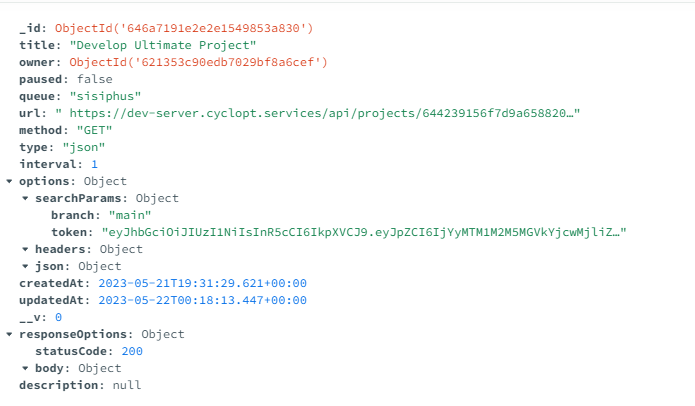
\includegraphics[width=0.9\textwidth]{./images/chapter4/api_doc.png}
	\caption[Παράδειγμα μίας τυπικής εγγραφής API.]{Παράδειγμα μίας τυπικής εγγραφής API.}
	\label{fig:api_doc}
\end{figure}\textbf{}

\begin{figure}[!ht]
	\centering
	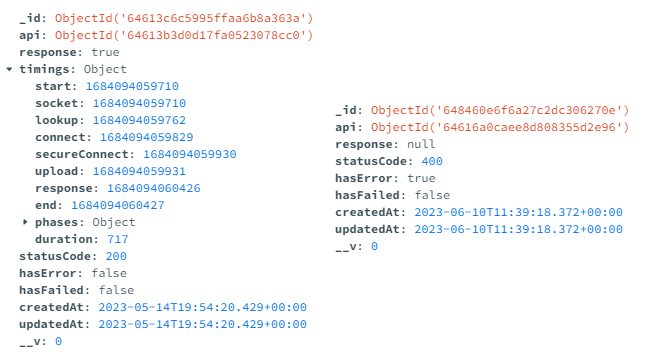
\includegraphics[width=0.9\textwidth]{./images/chapter4/response_docs.png}
	\caption[Παράδειγμα εγγραφών Responses σε αίτημα που πραγματοποιήθηκε επιτυχώς και σε αίτημα που απέτυχε λόγω σφάλματος στο σύστημα που μελετάμε.]{Παράδειγμα εγγραφών Responses σε αίτημα που πραγματοποιήθηκε επιτυχώς και σε αίτημα που απέτυχε λόγω σφάλματος στο σύστημα που μελετάμε.}
	\label{fig:response_docs}
\end{figure}\textbf{}

\section{Scheduler}
\label{section:lychte_scheduler}

Κύρια λειτουργία του συστήματος που υλοποιήσαμε είναι η αυτόματη παρακολούθηση του χρόνου λειτουργίας και απόκρισης ενός ιστότοπου/εφαρμογής. Για να γίνει αυτό θέλουμε ένα υποσύστημα που θα εκτελεί συνέχεια συγκεκριμένα κομμάτια κώδικα σε όσο το δυνατό πιο ακριβής χρονικές στιγμές.

Έχοντας ως ένα κοινό σημείο αναφοράς, τη Mongo βάση, μπορούμε να φτιάξουμε "έξυπνους" schedulers.
Κάθε scheduler θα είναι υπεύθυνος για περισσότερα από ένα apis, στα οποία θα κάνει requests, προκειμένου να δει αν είναι εν λειτουργεία και να ελέγξει την ορθότητα της επιστρεφόμενης απάντησης σε περίπτωση που ο χρήστης έχει ορίσει αναμενόμενη απάντηση. Πλέον και για την πιο οργανωμένη λειτουργία των schedulers προστίθεται ένα ακόμα collection στη βάση. Αυτό ονομάζεται Job (\autoref{fig:sample_job_document} και περιέχει τα εξής πεδία:

\begin{itemize}
    \item Name: η ονομασία του job που εκτελείται. Όπως θα δούμε και στη συνέχεια κάθε scheduler θα έχει παραπάνω από έναν τύπο jobs. Η βασική κατηγορία που θα εμφανίζεται κατά μεγαλύτερο βαθμό είναι η "api" και περιγράφει την εκτέλεση ενός αιτήματος σε ένα url και τον έλεγχο ορθότητάς του.
    \item Data: πληροφορία που είναι αποθηκευμένη στo collection api
    \item repeatInterval: ρυθμός επανάληψης του συγκεκριμένου job (σε ms)
    \item nextRutAt: ο χρόνος σε ms που θα πρέπει να ξανατρέξει το job
    \item lockedAt: πότε ξεκίνησε να εκτελείται (κλείδωσε) το συγκεκριμένο job
    \item Επιπλέον πεδία για την εύκολη αναγνώριση σφαλμάτων (debugging) όπως το (lastFinishedAt, lastRunAt)
\end{itemize}

\begin{figure}[!ht]
	\centering
	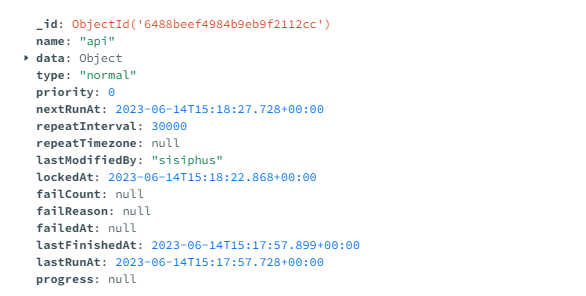
\includegraphics[width=0.8\textwidth]{./images/chapter4/sample_job_document.png}
	\caption[Παράδειγμα εγγραφής ενός \textbf{Job} στη βάση]{Παράδειγμα εγγραφής ενός \textbf{Job} στη βάση. Tο πεδίο \textit{lockedAt} έχει τιμή διάφορη του null, όταν το job ήδη εκτελείται.
		Το πεδίο \textit{nextRunAt} υπολογίζεται από το άθροισμα του χρόνου πλήρωσης της προηγούμενης εκτέλεσής του (\textit{lastFinishedAt}) και του interval. Στο πεδίο \textit{data}
		έχει αποθηκευμένη όλη την πληροφορία που χρειάζεται για να εκτελέσει το αίτημα για το οποίο δημιουργήθηκε το συγκεκριμένο job. Βάσει των πεδίων αυτών κυρίως κρίνεται το αν ο
		κεντρικός scheduler θα ξεκινήσει τη διεργασία}
	\label{fig:sample_job_document}
\end{figure}


Στο πλαίσιο του Lychte μπορούν να υπάρχουν παραπάνω από ένας scheduler που εκτελούν jobs τα οποία ορίζει κάθε φορά ο server. Προκειμένου να έχουμε παραπάνω από έναν scheduler δίνουμε σε κάθε έναν, ένα μοναδικό όνομα. Κάθε scheduler στη συνέχεια πηγαίνει και διαβάζει jobs που είναι αποθηκευμένα στο collection "όνομα-jobs", με αποτέλεσμα να έχεις καταμερισμό των jobs σε περισσότερους από έναν schedulers. Κάθε api πλέον αντιστοιχίζεται μονοσήμαντα σε έναν μόνο scheduler το όνομα του οποίου αποθηκεύεται και στο api που κρατάμε στη βάση κατά τη δημιουργία του. Ο scheduler αποφασίζεται από τον server ανάλογα με το πόσα apis εξυπηρετεί κάθε scheduler εκείνη την χρονική στιγμή.

Η λειτουργία των scheduler περιγράφεται στη συνέχεια. Αρχικά κάθε scheduler ψάχνει κάθε δέκα δευτερόλεπτα στη βάση ποια αιτήματα πρέπει να εκτελεστούν. Πιο συγκεκριμένα ελέγχει ποια jobs στο συγκεκριμένο collection εκτελούνται και πόσα από αυτά θα πρέπει θα πρέπει να εκτελεστούν. Αυτό μπορούμε να το γνωρίζουμε από πριν καθώς κάθε φορά που ξεκινάει ένα job αποθηκεύουμε το χρόνο που ξεκίνησε και υπολογίζουμε το πότε θα πρέπει να ξαναεκτελεστεί (start + repeatInterval). Όλα αυτά γίνονται μόνο εφόσον το job δεν είναι locked (έχει ξεκινήσει αλλά δεν έχει τελειώσει ακόμα). Έτσι αναγνωρίζουμε τις εξής περιπτώσεις χρονισμών:

\begin{itemize}
    \item Επιτυχής Εκτέλεση εντός χρονικού διαστήματος (\autoref{fig:perfect_request_cycle}). Κάθε φορά που έρχεται η στιγμή να ξαναεκτελεστεί το αίτημα έχει ήδη προλάβει να τελειώσει το προηγούμενο
    \item Καθυστερημένη Εκτέλεση αιτήματος (\autoref{fig:timeouts_request_cycle}): Αν κάποιο αίτημα αργήσει να εκτελεστεί, σε χρόνο μεγαλύτερο από το χρόνο που θα πρέπει να ξαναγίνει το αίτημα τότε βάζουμε timeout προκειμένου να λήξουμε πρόωρα το αίτημα και να μην υπάρξουν περαιτέρω καθυστερήσεις στα επόμενα αιτήματα που πρέπει να γίνουν εντός ορισμένου χρονικού διαστήματος
\end{itemize}

\begin{figure}[!ht]
	\centering
	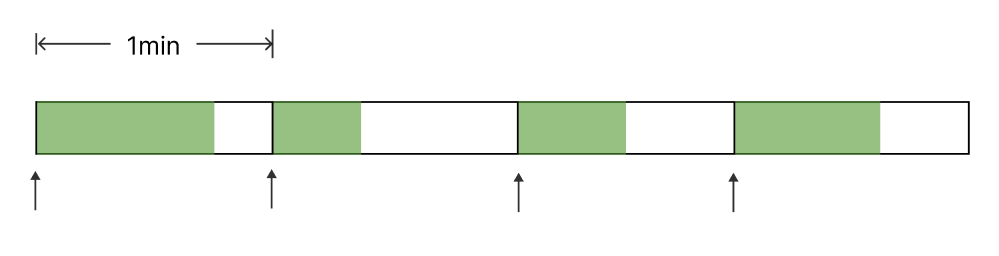
\includegraphics[width=0.8\textwidth]{./images/chapter4/perfect_request_cycle.png}
	\caption[Κύκλος Ζωής εκτέλεσης ενός επαναλαμβανόμενου Αιτήματος με ρυθμό επανάληψης ενός λεπτού]{Κύκλος Ζωής εκτέλεσης ενός επαναλαμβανόμενου Αιτήματος με ρυθμό επανάληψης ενός λεπτού}
	\label{fig:perfect_request_cycle}
\end{figure}

\begin{figure}[!ht]
	\centering
	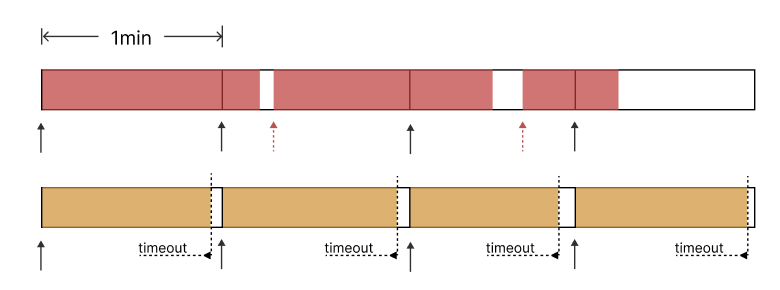
\includegraphics[width=0.8\textwidth]{./images/chapter4/timeout_request_cycle.png}
	\caption[Σύγκριση μη χρήσης και χρήσης timeouts στον κύκλο ζωής εκτέλεσης ενός αργού επαναλαμβανόμενου αιτήματος]{Σύγκριση μη χρήσης ή χρήσης timeouts στον κύκλο ζωής εκτέλεσης ενός αργού επαναλαμβανόμενου αιτήματος. Στην πρώτη περίπτωση το επόμενο αίτημα ξεκινάει μέσα σε χρόνο δέκα δευτερολέπτων από την στιγμή που εκτελέστηκε, με αποτέλεσμα οι χρονισμοί να μην είναι πάντα σταθεροί}
	\label{fig:timeouts_request_cycle}
\end{figure}



% 3.Oracle -> τρέχει τον RePAD2 και αν βρει anomally διαβάζει από το topic "usages" (json της μορφής (cpu: 30\%, ram: 90\% )).Αν κάποιο resource έχει αυξημένη ή μειωμένη χρήση στέλνει στο topic "updates" 

% Όταν κάνεις αναφορά στο oracle αν χρειαστεί να κάνεις επεξήγση του repad βάλε και τα ./images/chapter4/timeseries/repad2/experiment/subplots.png και ./images/chapter4/timeseries/repad2/experiment.png

% \begin{figure}[!ht]
% 	\centering
% 	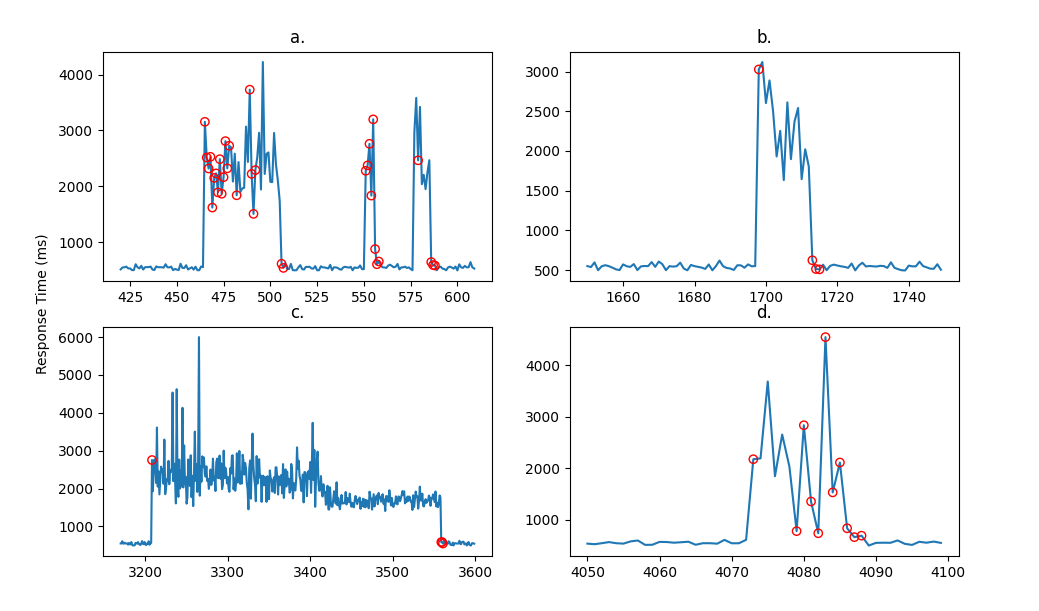
\includegraphics[width=0.9\textwidth]{./images/chapter4/timeseries_repad2_experiment_subplots.png}
% 	\caption[Αποτελέσματα χρήσης της CPU.]{Αποτελέσματα χρήσης της CPU.}
% 	\label{fig:repad2_experiments_subplots}
% \end{figure}

% \begin{figure}[!ht]
% 	\centering
% 	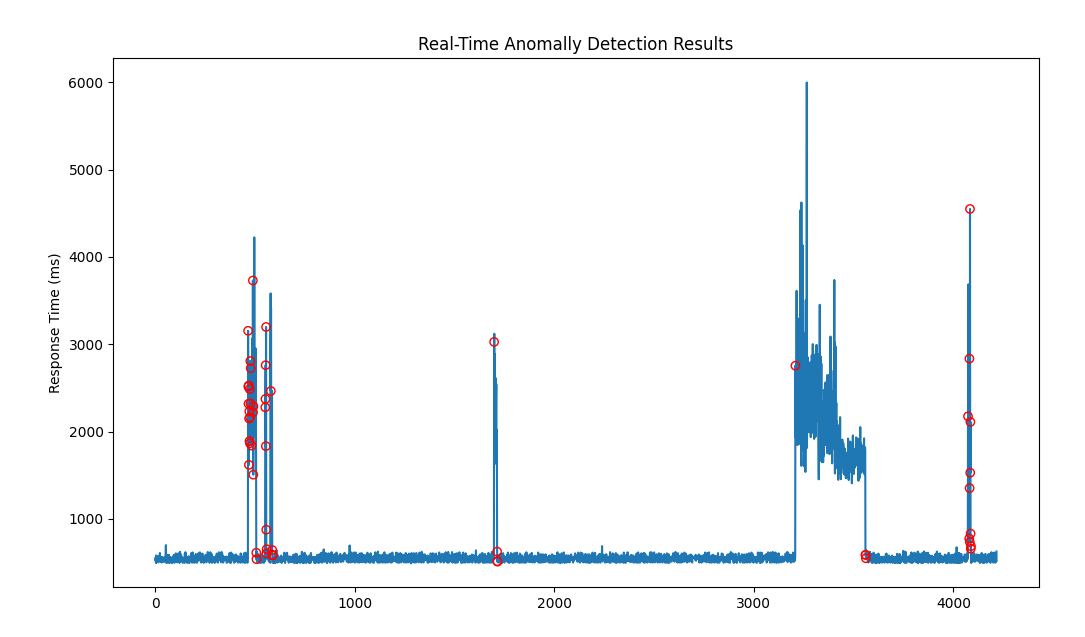
\includegraphics[width=0.9\textwidth]{./images/chapter4/timeseries_repad2_experiment.png}
% 	\caption[Αποτελέσματα χρήσης της CPU.]{Αποτελέσματα χρήσης της CPU.}
% 	\label{fig:repad2_experiments}
% \end{figure}

Όλα αυτά αφορούν αποκλειστικά τη λειτουργία του backend του συστήματος. Πέρα από αυτά
θα πρέπει να υπάρχει μία γραφική διεπαφή, μέσω της οποίας, κάθε χρήστης θα μπορεί να δει τα δεδομένα που παράγονται
από τη χρήση του συστήματός.

Το σύστημα όμως, όπως είναι τώρα, δεν είναι σε θέση να μπορεί να δείχνει επαρκώς γρήγορα ιστορικά δεδομένα. Αν υποθέσουμε ότι έχουμε ένα Api που θέλουμε να ελέγχουμε κάθε
λεπτό, στο τέλος της ημέρας θα έχουν μαζευτεί από αυτό και μόνο 1.440 εγγραφές. Αν αυτά συνεχίζουν να μαζεύονται, τότε ακόμα και τα πιο απλά queries στο μοντέλο των αποκρίσεων θα καθυστερούν, καθιστώντας έτσι την εφαρμογή αργή. Για την αποφυγή συσσώρευσης περιττής, μετά από ορισμένο χρονικό διάστημα, πληροφορίας, έχουμε βάλει επιπρόσθετα σε κάθε scheduler ένα ακόμα job που αφορά
τον καθαρισμό της βάσης από εγγραφές που προέρχονται από το καθένα. Η διεργασία αυτή τρέχει μία φορά την εβδομάδα. Κάθε φορά που εκτελείται ψάχνει τα Apis ανάλογα με τον scheduler στον οποίο τρέχει.
Έπειτα μαζεύει όλες τις αποκρίσεις που σχετίζονται με το κάθε Api ξεχωριστά και ξεκινάει τους υπολογισμούς. Τα δεδομένα που αντλούνται στο πλαίσιο αυτής της διεργασίας, στο τέλος, διαγράφονται από τη βάση, ώστε ολα τα αιτήματα στη βάση να εκτελούνται πιο γρήγορα και αποδοτικά. Σβήνοντας όμως πληροφορία, χάνουμε την ιστορικότητα των δεδομένων μας, με αποτέλεσμα να χάνουν και οι χρήστες μία πιο γενική εικόνα των ελέγχων που έχουν πραγματοποιηθεί. Στο σημείο αυτό εισάγεται μία άλλης μορφής βάση δεδομένων, η Google Cloud Storage.

Πριν σβήσουμε δεδομένα που κρίνουμε ότι δεν είναι απαραίτητο να υπάρχουν στη βάση, αλλά έχουν αξία για ιστορική ανάλυση, τα μεταφέρουμε στο Cloud Storage της Google, υπό μορφή αρχείων.
Με τον τρόπο αυτό κερδίζουμε χώρο, στη κεντρική Mongo βάση, στη λειτουργία της οποίας στηρίζεται όλο το σύστημα, και γενικά απόδοση καθώς έχει καλύτερες ταχύτητες στο σύνολο (\autoref{fig:lychte_server_scheduler}). 

\begin{figure}[!ht]
	\centering
	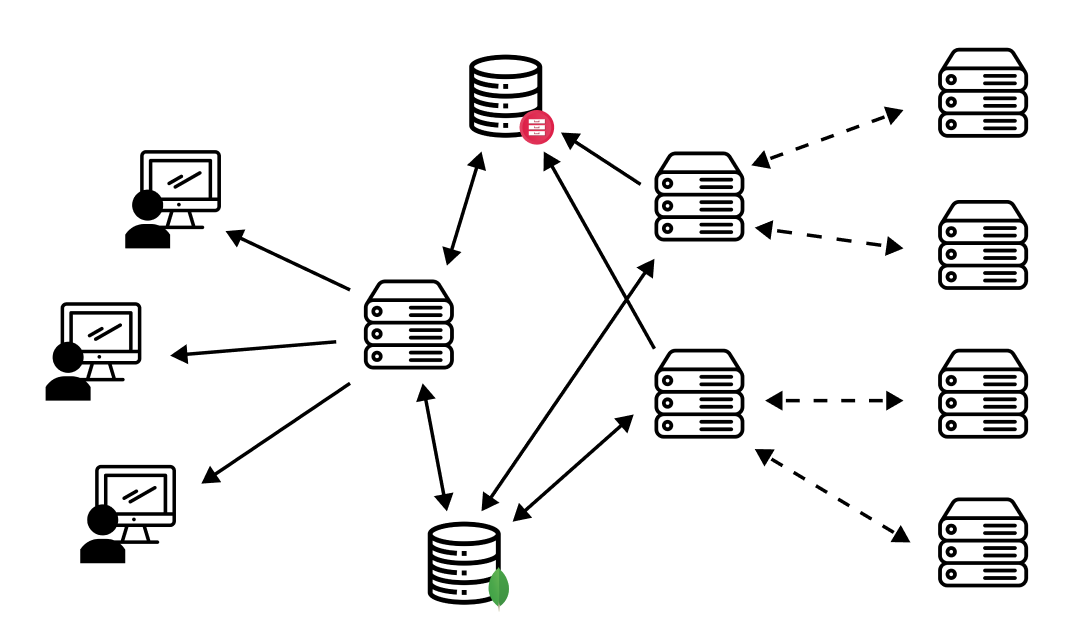
\includegraphics[width=0.8\textwidth]{./images/chapter4/lychte-third-implementation-full.png}
	\caption[Διάγραμμα λειτουργίας Server-Schedulers.]{Διάγραμμα λειτουργίας Server-Schedulers.}
	\label{fig:lychte_server_scheduler}
\end{figure}

Στη συνέχεια θα αναφερθούμε πιο συγκεκριμένα στς βήματα που ακολουθούμε προκειμένου να καθαρίσουμε τη βάση:

\begin{enumerate}
	\item Συλλογή όλων των Responses που υπάρχουν αποθηκευμένα στη βάση, μέχρι μία μέρα πριν την εκτέλεση της διεργασίας καθαρισμού. Αυτό γίνεται προκειμένου να σιγουρευτούμε ότι υπάρχει πάντα πληροφορία στη βάση για την προηγούμενη ημέρα που μπορούμε να δείξουμε.
	\item Δημιουργία δύο διαφορετικών πινάκων, ενός που αποθηκεύει τους χρόνους διάρκειας των αιτημάτων και ενός που περιέχει Boolean μεταβλητές σχετικά με το αν τα αιτήματα γίνονται επιτυχώς ή όχι.
	\item Στη συνέχεια, για κάθε μέρα στην οποία έχουμε εγγραφές Responses, υπολογίζουμε και αποθηκεύουμε στατιστικά σχετικά με τη μέση τιμή, διάμεσο και τυπική απόκλιση διάρκειας των αιτημάτων.
	\item Στο τέλος της διαδικασίας αποθηκεύονται τρία αρχεία για κάθε Api. Ένα στο οποίο περιέχονται τα responses όπως ακριβώς ήταν αποθηκευμένα στη mongodb (σε αρχείο της μορφής \textbf{"../apiId/raw-responses/MM-DD-YYYY.json"}), ένα που περιέχει τους πίνακες που περιγράψαμε στο δεύτερο βήμα (\textbf{"../apiId/\hyp{}raw-values/MM-DD-YYYY.avro"}) και τέλος, ένα αρχείο που περιέχει κάποια χρήσιμα στατιστικά για κάθε μέρα που εντοπίστηκε, όπως περιγράφεται στο βήμα τρία (\textbf{"../apiId/statistics.avro"}) 
\end{enumerate}

Επειδή τα αρχεία που περιέχουν στατιστικά για κάθε μέρα χρησιμοποιούνται αρκετά συχνά από τη γραφική διεπαφή του Lychte για την παρουσίαση ιστορικών δεδομένων του υπό μελέτη Api, κρίναμε απαραίτητη τη χρήση ενός διαφορετικού τύπου αρχείου σε σχέση με
τον κλασσικό και ευρέως διαδεδομένο στο διαδίκτυο τύπο JSON, το AVRO, για να κερδίσουμε ως προς τον αποθηκευτικό χώρο αλλά και την ταχύτητα ανάγνωσης. Αξίζει να σημειωθεί ότι ένα αρχέιο avro σε σχέση με ένα αρχείο json που περιέχουν ακριβώς την ίδια
πληροφορία, για τα στατιστικά στα οποία αναφερόμαστε, είναι 70\% περίπου μικρότερο σε μέγεθος (json αρχείο 250Μb, avro αρχείο 75Μb)
Ο λόγος που μπορούμε να χρησιμοποιήσουμε avro αρχεία είναι ότι η μορφή της αποθηκευμένης πληροφορίας παραμένει ίδια και δεν αλλάζει. Πιο συγκεκριμένα, τα schemas που χρησιμοποιούνται στα αρχεία \textbf{"raw-values/MM-DD-YYYY.avro"} και \textbf{"statistics.avro"}
φαίνονται στο \autoref{fig:avro_types}.

\begin{figure}[!ht]
	\centering
	\makebox[\textwidth][c]{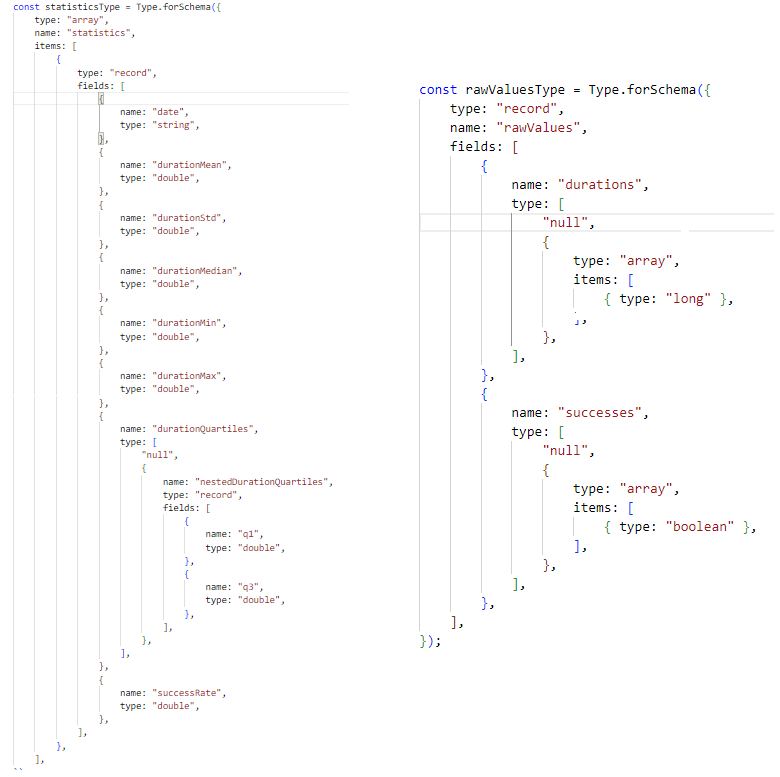
\includegraphics[width=0.87\textwidth]{./images/chapter4/avro_types.png}}
	\caption[Schemas πληροφορίας που αποθηκεύουμε σε avro αρχεία]{Schemas πληροφορίας που αποθηκεύουμε σε avro αρχεία. Το πρώτο αφορά τα statistics που αποθηκεύονται και αποτελείται από ένα array από objects, τα fields των οποίων σχετίζονται σε μετρικές στατιστικής φύσης. Το δεύτερο schema χαρακτηρίζει τα raw-values που αποθηκεύουμε και αποτελείται από ένα object με δύο arrays}
	\label{fig:avro_types}
\end{figure}

\section{Krosswalk}
\label{section:lychte_krosswakl}

Το τρίτο αυτό υποσύστημα μπορεί να υπάρχει εφόσον ο ιστότοπος/εφαρμογή που θέλουμε να ελέγξουμε έχει δημιουργηθεί με εργαλεία docker. Αποτελεί δηλαδή ένα docker container. Το ίδιο έχει πάλι τη μορφή docker container και είναι υπεύθυνο για την συλλογή logs των πόρων του container που θέλουμε να μελετήσουμε και την αποστολή τους σε μία ουρά kafka προκειμένου να έχουμε persistent δεδομένα από τη λειτουργία του. Το krosswalk αποτελεί container που θα πρέπει ο ίδιος ο χρήστης να εγκαταστήσει και να εκτελέσει στο δικό του docker, ώστε να βρίσκεται "δίπλα" σε αυτό που θέλει να ελέγχετε.

Το krosswalk αποτελεί ένα container, που περιέχει ένα εκτελέσιμο αρχείο, το οποίο προήλθε από το "χτίσιμο" κώδικα γραμμένου σε Rust. H γλώσσα πραγραμματισμού Rust επιλέχθηκε κατά κύριο λόγο για την ασφάλεια μνήμης, τις δυνατότητες παράλληλου προγραμματισμού, την αποδοτικότητα που προσφέρει καθώς και τη δυνατότητα δημιουργίας εκτελέσιμων αρχείων (αρχείων που εκτελεί ο υπολογιστής και δεν μπορούν να διαβαστούν από τον άνθρωπο). Αξίζει να σημειωθεί ότι για να κάνουμε έλεγχο ενός συγκεκριμένου container θα πρέπει να γνωρίζουμε το container id του docker container. Αυτό το γνωρίζει μόνο ο χρήστης και το προσθέτει σαν μεταβλητή περιβάλλοντος στο dockerfile του container που περιέχει το krosswalk.

Η βασική λειτουργία του είναι να εκτελεί την εντολή \textit{\textbf{"docker stats cntrId"}} κάθε n (=10) δευτερόλεπτα και να υπολογίζει το ποσοστό χρήσης CPU και RAM του container σε σχέση πάντα με τους διαθέσιμους πόρους που του προσφέρουμε. Αν π.χ. παρέχουμε 0.5cpu και η εκτέλεση της παραπάνω εντολής μας λέει ότι κάνουμε χρήση του 50\% της cpu, τότε καταλαβαίνουμε αμέσως ότι κάνουμε 100\% χρήση της διαθέσιμης cpu, καθώς το docker δίνει το ποσοστό κατανάλωσης όχι ανάλογα με τους διαθέσιμους πόρους αλλά με ποσοστό χρησης της φυσικής cpu του μηχανήματος που τρέχει το container (κάθε 100\% αντιστοιχεί σε 1 physical core). Κάτι παρόμοιο εφαρμόζεται για τον υπολογισμό του ποσοστού χρήσης της μνήμης (RAM). Αυτά στη συνέχεια αποστέλλονται σαν events σε μία ουρά kafka στο topic usages. Εδώ αξίζει να σημειωθεί ότι κάθε φορά που στέλνουμε ένα μήνυμα βάζουμε σαν κλειδί το id του api που αντιστοιχεί στο συγκεκριμένο έλεγχο προκειμένου να μπορούμε να ξεχωρίζουμε ποια usages ανήκουν σε ποια apis. Πέρα από λειτουργίες Kafka Producer θα πρέπει να διαθέτει και λειτουργίες Consumer προκειμένου να τροποποιεί τα resources ανάλογα με τα μηνύματα που θα δέχεται από το επόμενο κατά σειρά υποσύστημα Oracle.

Έτσι στην αρχή λειτουργίας του Krosswalk ξεκινάμε δύο threads, ένα που εκτελεί την παραπάνω διεργασία και ένα που διαβάζει κάθε n (=10) δευτερόλεπτα μηνύματα από τον topic updates, μόνο εφόσον αυτά έχουν σαν κλειδί το id του api που ελέγχουμε. Ανάλογα με το μήνυμα που δέχεται κάθε φορά εκτελεί την εντολή 
\textit{\textbf{"docker update --cpus x --memory y cntrId"}} αυξάνοντας/μειώνοντας τη cpu κατά 0.5 πυρήνες και τη μνήμη κατά 0.5gb. 

\section{Oracle}
\label{section:lychte_oracle}

Αποτελεί το τέταρτο και τελευταίο υποσύστημα του Lychte. Είναι υπεύθυνο για αναγνώριση ανωμαλιών καθώς και την λήψη αποφάσεων σχετικά με το αν θα πρέπει να γίνει αύξηση ή μείωση των διαθεσίμων πόρων, εφόσον έχει εγκατασταθεί το Krosswalk, στο υπό μελέτη σύστημα.

Όπως προαναφέραμε, πριν γίνει οποιαδήποτε τροποποίηση στο σύστημα που μελετάμε κάθε φορά, θα πρέπει πρώτα να βρούμε σημεία στη χρονοσειρά των αποκρίσεων ενός συστήματος που δηλώνουν απόκλιση από το φυσιολογικό. Για να πετύχουμε κάτι τέτοιο χρησιμοποιήσαμε τον αλγόριθμο RePAD2 \cite{lee2023repad2}. Τα βήματα του αλγορίθμου μπορούμε να τα δούμε και στο \autoref{fig:repad2}. Ουσιαστικά εκπαιδεύουμε ένα LSTM με τις τελευταίες τρεις τιμές μάθε φορά της προαναφερθείσας χρονοσειράς και κάνουμε προβλέψεις για την τιμή της τωρινής. Στη συνέχεια υπολογίζουμε ένα δείκτη σφάλματος που συνυπολογίζει τη σχετική διαφορά των τελευταίων τρία κατα σειρά τιμών από τις προβλεπόμενες. Αν αυτό ξεπερνάει ένα threshold (η τιμή του οποίου υπολογίζεται εκ νέου σε κάθε επανάληψη) τότε θεωρούμε ότι υπάρχει εν δυνάμει ανώμαλο σημείο στη χρονοσειρά. Στην περίπτωση που αυτό υπάρξει δημιουργούμε ένα καινούργιο μοντέλο LSTM το οποίο εκπαιδεύεται στα τελευταία τρία σημεία και υπολογίζονται εκ νέου οι μεταβλητές που χρειαζόμαστε (νέα προβλεπόμενη τιμή, νέα τιμή threshold, νέα τιμή σχετικού σφάλματος).

\begin{figure}[!ht]
	\centering
	\makebox[\textwidth][c]{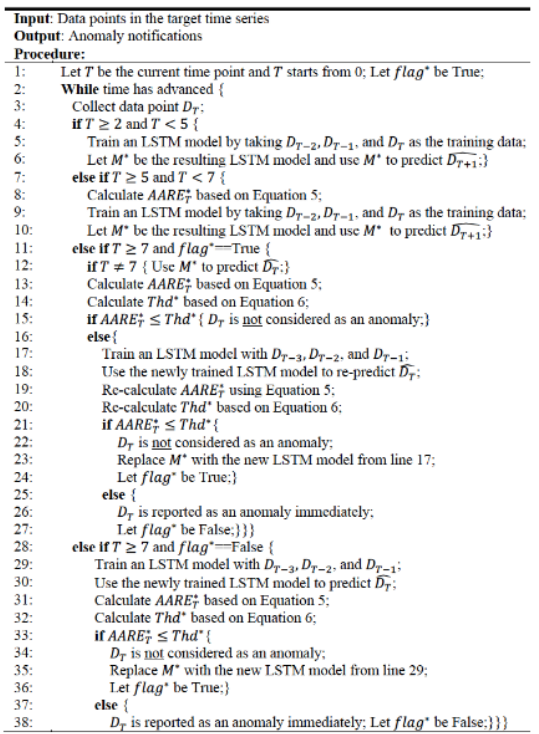
\includegraphics[width=1\textwidth]{./images/chapter4/repad2.png}}
	\caption[Ανάλυση κώδικα REPAD2]{Ανάλυση κώδικα REPAD2}
	\label{fig:repad2}
\end{figure}

Από την παραπάνω λειτουργία παρατηρούμε γρήγορα ότι ένα από τα πλεονεκτήματα του αλγορίθμου είναι το γεγονός ότι δε χρειάζεται μεγάλο αριθμό training data, καθώς για να ξεκινήσει τη λειτουργία του χρειάζεται τρία σημεία κάθε φορά. Στην πραγματικότητα ο εντοπισμός ανώμαλων σημείων γίνεται από τη στιγμή που έχουμε 7 και παραπάνω ενδείξεις καθώς μέχρι το έβδομο σημείο γίνονται οι πρώτοι ακόμα υπολογισμοί των σχετικών σφαλμάτων που θα χρειαστούν σε επόμενα βήματα. Ένα ακόμα πλεονέκτημα είναι ότι τα δεδομένα που του δίνουμε στο στάδιο της εκπαίδευσης δεν έχουν labels. Αναφερόμαστε δηλαδή σε αμιγώς unsupervised learning. Τέλος η «επανεκπαίδευση» δεν γίνεται σε κάθε επανάληψη αλλά μόνο όταν κρίνεται ότι υπάρχει σημείο που αποκλίνει από τη φυσιολογική τάση της χρονοσειράς. Αξίζει να αναφερθεί ότι η διαδικασία δημιουργίας καινούργιου LSTM ειναι πολύ γρήγορη (0.2 δευτερόλεπτα κατά μέσο όρο) με αποτέλεσμα οι προβλέψεις που κάνουμε να πλησιάζουν συμπεριφορά real time (ακόμα και στην περίπτωση που πρέπει να ξαναφτιάξουμε καινούργιο μοντέλο).

Ο παραπάνω αλγόριθμος, στο πλαίσιο αυτής της διπλωματικής αναφοράς, υλοποιήθηκε με χρήση της προγραμματιστικής γλώσσας python και κατά κύριο λόγω με βιβλιοθήκες αυτής όπως οι pandas και numpy για την αποθήκευση/τροποποίηση δεδομένων και η tensorflow για τη δημιουργία, διαχείρηση, αποθήκευση machine learning μοντέλων. Η αποθήκευση των δεδομένων που χρειάζονται σε μελλοντικά στάδια του αλγορίθμου όπως είναι ο δείκτης σχετικού σφάλματος και οι προβλέψεις που κάνουμε σε κάθε βήμα αποθηκεύονται στη βάση mongo, στο αντίστοιχο collection responses κάθε φορά, τροποποιώντας έτσι ελάχιστα το schema που είχαμε ορίσει στην αρχή του κεφαλαίου. Το python script έχει έναν mini scheduler που ξεκινάει τον επαναληπτικό αλγόριθμο. Αυτός καλείτε κάθε m (=10 δευτερόλεπτα) για κάθε api που θέλουμε να κάνουμε real time anomaly detection).

Αφού γίνει η αναγνώριση «σφάλματος» στο υπό μελέτη σύστημα θα πρέπει να γίνεται και διόρθωση αυτού. Σε αυτό το σημείο έρχεται το Krosswalk και η Kafka ουρά στην οποία κρατάμε δεδομένα για τη λειτουργία του συστήματος (εφόσον όπως έχουμε ήδη αναφέρει αποτελεί docker container και έχει εγκατασταθεί το Krosswalk σε ένα container εντός του υπό μελέτη συστήματος). Συνεπώς μετά την αναγνώριση λάθους το python script ξεκινάει να λειτουργεί σαν Kafka Consumer. Διαβάζει events από το topic usages μέχρι να βρει κάποιο που προέρχεται από το api που αναλύει εκείνη τη στιγμή. Αν εντός k δευτερολέπτων δε λάβει απάντηση συνεχίζει κανονικά τη λειτουργία του σε μια επόμενη επανάληψη. Αν λάβει κάποιο μήνυμα τότε ανάλογα με το ποσοστό χρήσης της μνήμης και της CPU στέλνει ανάλογα μηνύματα για την αύξηση ή μείωση του καθενός ξεχωριστά. Πιο συγκεκριμένα αν το ποσοστό χρήσης ξεπερνά το 90\% τότε αυξάνει τους πόρους και αν είναι κάτω του 10\%, τους μειώνει κατά μια μονάδα κάθε φορά (0.5 πυρήνες για τη cpu και 0.5gb για τη μνήμη). Για να μεταφερθεί η πληροφορία τροποποίησης των πόρων στο Krosswalk, το Oracle στέλνει ένα event στο topic updates με συγκεκριμένες κάθε φορά εντολές.

Προκειμένου να δούμε καλύτερα τη λειτουργία του αλγορίθμου RePAD2 και να μελετήσουμε την αποτελεσματικότητα του στο δικό μας σύστημα έχουμε πάρει πραγματικά δεδομένα απο χρονικές αποκρίσεις ενός συστήματος και τον εφαρμόσαμε πάνω σε αυτά. Οι αποκρίσεις φαίνονται στο \autoref{fig:repad2_experiments}. Με κόκκινα κυκλάκια σηματοδοτούμε τα σημεία στα οποία η εφαρμογή του αλγορίθμου εντοπίζει ανώμαλα σημεία. Για να γίνουν πιο εμφανή τα σημεία που εντοπίστηκαν, στο \autoref{fig:repad2_experiments_subplots} μπορούμε να τα δούμε σε μεγέθυνση. Αξίζει να σημειωθεί ότι και στις έξι περιπτώσεις που έχουμε ανώμαλα σημεία, τέτοια δηλαδή που αποκλίνουν από τους φυσιολογικούς χρονισμούς που παρατηρούνται, ο εντοπισμός γίνεται τόσο στην αρχή της αύξησης του φόρτου του υπο μελέτη συστήματος όσο και στη μείωση αυτού. Στις πρώτες τρεις μάλιστα περιπτώσεις αύξησης του φορτίου βλέπουμε ότι παρατηρούνται περισσότερα από ένα συνεχόμενα σημεία που αναγνωρίζονται ως ανώμαλα. Κάτι το οποίο σε επόμενες περιπτώσεις δε συμβαίνει αφού ο εντοπισμός γίνεται στην αρχή και στο τέλος της τροποποίησης του φορτίου. Αυτό γίνεται διότι ο τρόπος που υπολογίζεται το όριο απόφασης (decision threshold) εμπεριέχει όλες τις προηγούμενες τιμές σχετικού λάθους. Με αποτέλεσμα όσο περισσότερα δεδομένα υπάρχουν τόσο πιο ανθεκτικός να είναι σε μικρότερες μεταβολές.

\begin{figure}
    \centering
	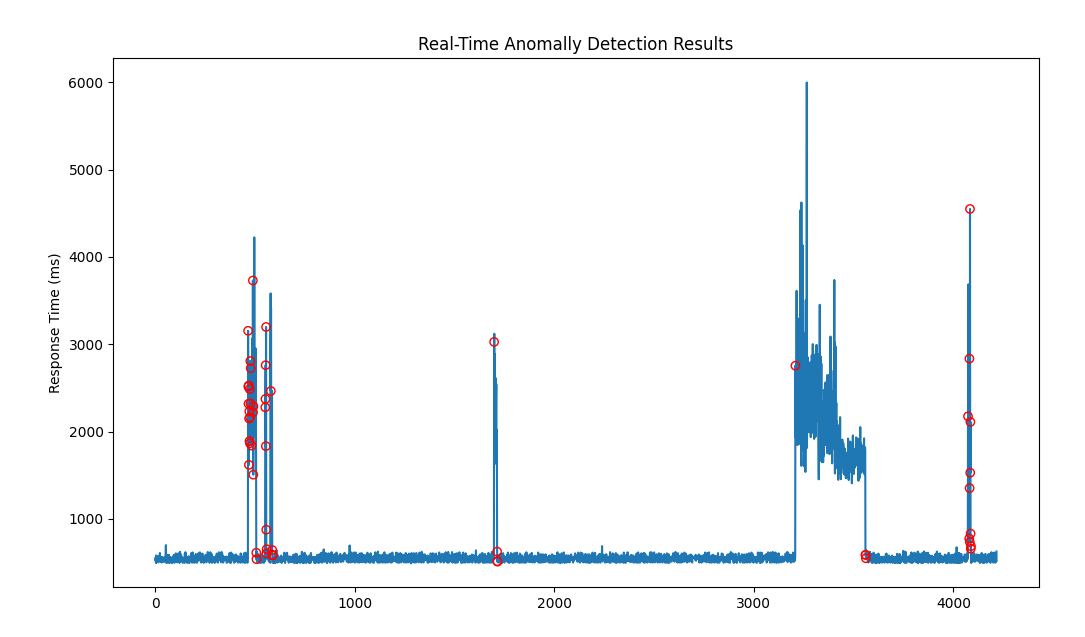
\includegraphics[width=0.9\textwidth]{./images/chapter4/timeseries_repad2_experiment.png}
	\caption[Χρονοσειρά αποκρίσεων ενός συστήματος που προήλθε απο τη χρήση του συστήματος Lychte. Με κόκκινο φαίνονται τα ανώμαλα σημεία που εντοπίστηκαν απο τη χρήση του RePAD2.]{Χρονοσειρά αποκρίσεων ενός συστήματος που προήλθε απο τη χρήση του συστήματος Lychte. Με κόκκινο φαίνονται τα ανώμαλα σημεία που εντοπίστηκαν απο τη χρήση του RePAD2.}
	\label{fig:repad2_experiments}
\end{figure}

\begin{figure}
	\centering
	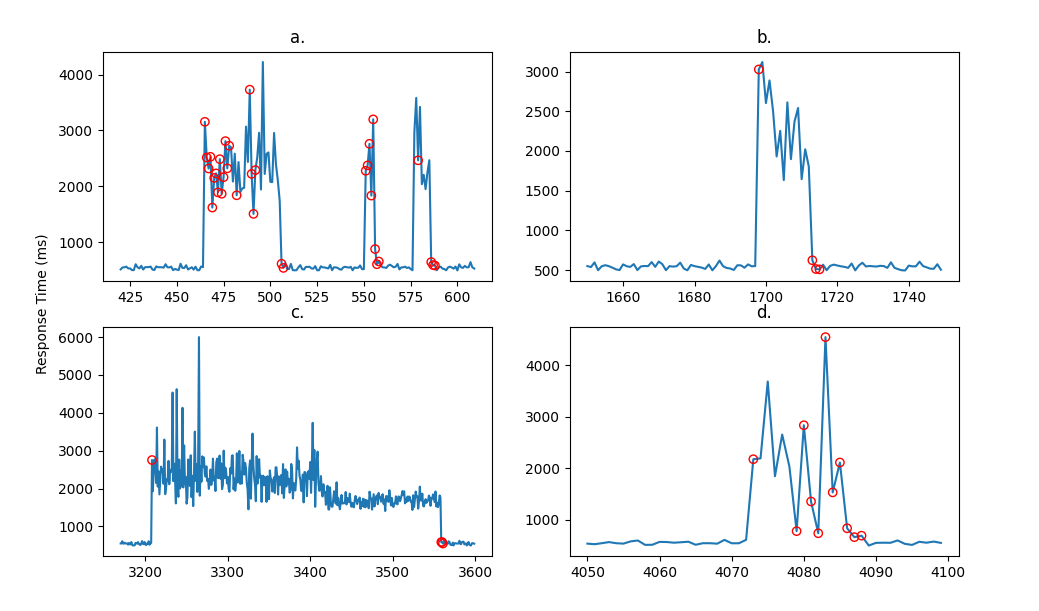
\includegraphics[width=0.9\textwidth]{./images/chapter4/timeseries_repad2_experiment_subplots.png}
	\caption[Εντοπισμένα σημεία ανωμαλιών σε μεγέθυνση.]{Εντοπισμένα σημεία ανωμαλιών σε μεγέθυνση.}
	\label{fig:repad2_experiments_subplots}
\end{figure}

\newevenside

% % chapter 5 = Επίδειξη Συστήματος
% - Παρουσίαση εικόνων από website
% - Εξήγεισαι τι δείχνουν και λειτουργικότητα

% ****ακράιες συνθήκες λειτουργίας συστήματος - πειράματα*******
% 	σε local βάση (πειράματα για 1ώρα) - κράτα σε αρχεία usage statiustics για το node process (ram, cpu, ....) ανά λεπτό
%	1) 50 apis σε ένα worker
%	2) 100 apis σε ένα worker
%	3) 200 apis σε ένα worker
%	4) 400 apis σε ένα worker
%	5) 400 apis σε ένα worker
% για καθένα από τα παραπάνω υπολόγιζε μέσο βαθμό απόκλισης από το expected interval και βάλε από δίπλα αποτελέσματα ram usage και cpu usage των threads εφόσον γίνεται


\newevenside
%\newevenside

\renewcommand{\bibname}{Βιβλιογραφία}
\bibliography{
	./bibliography/chapter1.bib,
	./bibliography/chapter2.bib,
	./bibliography/chapter3.bib
}

\end{document}

